% H1 report (XeLaTeX)
\documentclass[11pt,a4paper]{article}
\usepackage{fontspec}
\setmainfont{lmroman10}[Extension=.otf,UprightFont=*-regular,BoldFont=*-bold,ItalicFont=*-italic,BoldItalicFont=*-bolditalic]
\newfontfamily\cyrfont{DejaVuSerif}[Extension=.ttf,BoldFont=DejaVuSerif-Bold,ItalicFont=DejaVuSerif-Italic,Scale=0.88]
\usepackage[margin=2.2cm]{geometry}
\usepackage{amsmath,amssymb,amsthm,mathtools,bm}
\usepackage{graphicx,booktabs,tabularx,array,multirow,enumitem,xcolor}
\usepackage[most]{tcolorbox}
\usepackage{tikz}
\usetikzlibrary{arrows.meta,positioning,shapes.geometric,fit}
\usepackage[colorlinks,linkcolor=blue!50!black,citecolor=green!35!black,urlcolor=blue!50!black]{hyperref}
\setlist{itemsep=1pt,topsep=2pt}
\numberwithin{equation}{section}

\newtheorem{theorem}{Theorem}[section]
\newtheorem{lemma}[theorem]{Lemma}
\newtheorem{proposition}[theorem]{Proposition}
\newtheorem{corollary}[theorem]{Corollary}
\theoremstyle{definition}
\newtheorem{definition}[theorem]{Definition}
\newtheorem{assumption}[theorem]{Assumption}
\theoremstyle{remark}
\newtheorem{remark}[theorem]{Remark}
\newtheorem{example}[theorem]{Example}

\newcommand{\E}{\mathbb E}\newcommand{\R}{\mathbb R}\newcommand{\N}{\mathbb N}\newcommand{\Prob}{\mathbb P}
\newcommand{\norm}[1]{\lVert #1\rVert}\newcommand{\abs}[1]{\lvert #1\rvert}\newcommand{\ip}[2]{\langle #1,#2\rangle}
\newcommand{\Dmax}{\Delta_{\max}}\newcommand{\Dcp}{\Delta_{\rm cp}}
\newcommand{\cN}{\mathcal N}\newcommand{\cG}{\mathcal G}\newcommand{\cF}{\mathcal F}\newcommand{\cS}{\mathcal S}
\newcommand{\Unif}{\mathrm{Unif}}\newcommand{\TV}{\mathrm{TV}}\newcommand{\tmix}{t_{\rm mix}}
\newcommand{\Sph}{\mathbb S^{d-1}}\newcommand{\Ball}{\mathbb B}
\newcommand{\hatm}{\hat m_\gamma}\newcommand{\supp}{\operatorname{supp}}
\newcommand{\status}[1]{\textsf{\small[#1]}}
\newcommand{\ok}{\textcolor{green!45!black}{\textsf{proven}}}
\definecolor{hl}{HTML}{2a78d6}
\tcbset{card/.style={colback=blue!2,colframe=blue!45!black,boxrule=0.6pt,arc=2pt,left=6pt,right=6pt,top=4pt,bottom=4pt,fonttitle=\bfseries}}

\title{\textbf{H1: the structure of the class $\cN(\Delta,\tau,\gamma)$\\ and a correct definition of $\Dmax$}\\[2pt]
\large Local study report}
\author{}
\date{11 November 2026}

\begin{document}
\maketitle

\tableofcontents

%=====================================================================================================
\setcounter{section}{-1}
\section{Summary card}\label{sec:card}
\begin{tcolorbox}[card,title={H1 in one page}]
\textbf{Hypothesis.} Condition (2) constrains only $m=\E_\pi\delta$; for fixed $\gamma$ the class contains non-trivial ``Bessel'' $m$,
for all $\gamma\le\gamma_0$ it forces $m\equiv\mathrm{const}$; without a fixed budget $\Dmax=\infty$, so $T$ and the query protocol must enter the definition.

\textbf{Verdict: confirmed in a refined form.} The four mathematical claims are proven (for bounded measurable noise, with condition (2) read
for a.e.\ $x$), the algorithmic ones under the conditions stated below and in \S\ref{sec:verdict} ($\gamma\le\varepsilon/(4M)$ for the fixed-radius class; expectation variant, with $\varepsilon\to\beta\varepsilon$ for the probability variant); two refinements: (i) \emph{two radii} $\gamma_1,\gamma_2$ with $\gamma_1/\gamma_2\notin\{j_{d/2,k}/j_{d/2,l}\}$ already force $m\equiv{\rm const}$ (proven on $\R^d$; on a ball only cited), but in high dimension a second radius $\gamma_2\gtrsim\gamma_1$ is quantitatively almost useless;
(ii) the protocol matters: if idle rounds are free, $\tau$ drops out of the problem entirely (Prop.~\ref{prop:wait}).

\textbf{Main result (one formula).} With batching over states and a burn-in of $t_0=\tau\lceil\log_2(16R\sqrt d\,\Delta/(\gamma\varepsilon))\rceil_+$ rounds, $\E f(\bar x)-f^*\le\varepsilon$ after
\[
T(\Delta)=\Big\lceil\tfrac{145}{4}\tfrac{M^2R^2}{\varepsilon^2}\Big\rceil\Big(\Big\lceil \tfrac{2d^2}{d-1}+(2d+8\tau-3)\,\tfrac{d\Delta^2}{M^2\gamma^2}\Big\rceil+t_0\Big)
=O\!\Big(\tfrac{R^2}{\varepsilon^2}\big[dM^2+(d+\tau)\tfrac{d\Delta^2}{\gamma^2}\big]+\tau\log\Big)
\]
rounds, for every $\Delta<\infty$, provided $\gamma\le\varepsilon/(4M)$ (Thm.~\ref{thm:alg}; expectation variant). Hence $\Dmax=\infty$ without a budget \emph{for the all-radii class} (unconditionally: there $\E_\pi\delta={\rm const}$ and the algorithm chooses its radius) \emph{and for the fixed-radius class with $\gamma\le\varepsilon/(4M)$}; for the fixed-radius class with $\gamma>\varepsilon/(4M)$ nothing is proven (H6). Further,
$\Dmax^{\E}(T)\ \ge\ \frac{\varepsilon\gamma}{R}\sqrt{T/\big(74.5\,(2d+8\tau-3)\,d\big)}$ for $\gamma\le\varepsilon/(4M)$ and $T\ge 2T_1(\Delta)$, so $T\gtrsim\tau(MR/\varepsilon)^2\log$ --- the \emph{first branch} of the lower half of H2, proven outside the regime $\tau\gtrsim T$. In the probability variant of Def.~\ref{def:dmax} the same holds with $\varepsilon\to\beta\varepsilon$ (Markov's inequality, Cor.~\ref{cor:prob}).

\textbf{What it implies for the problem.} Without a budget the threshold is degenerate, so a non-degenerate $\Dmax$ carries the round budget $T$ and the $q$-query protocol (one chain step per round, idle rounds counted, exogenous chain), and the ``expected picture'' is a statement about the \emph{complexity-preserving level} $\Dcp(C)=\Dmax(T=C\,T_0)$. In the expectation variant, $\Dcp(C)\ge M\gamma/\sqrt{2d+8\tau-3}$ for $\gamma\le\varepsilon/(4M)$ and $C\ge\frac{149}4(6+t_0/d)$ (e.g.\ $C=261$ when $\tau\lceil\log_2(16MR/\varepsilon)\rceil\le d$); this is the lower side of the ``expected picture'' $M\gamma/\sqrt d$, and only the lower side is proven here (Def.~\ref{def:dmax}, Cor.~\ref{cor:cp}). In the all-radii class, (2) for all $\gamma\le\gamma_0$ reduces to ``$\E_\pi\delta(x,\cdot)={\rm const}$'' (Thm.~\ref{thm:allgamma}); there $\gamma$ leaves the class and becomes an algorithm parameter.

\textbf{Numerics.} E1.1, E1.3, E1.4 (5 seeds each) agree with their predictions: Bessel zeros give MC-level bias, off-zero bias matches $\Delta t\Psi_d(t)/d$; the tuned wave at a second radius follows $\Delta|\omega||\Psi_d(\gamma_2|\omega|)|$; the batched second moment equals the exact $A+S\,(1+\alpha)/(1-\alpha)$ within $1.41\%$ (additive in $d$ and $\tau$). E1.2 (logistic regression): the target is reached for every $\Delta$, and the budget is consistent with $\Delta^2$ --- the slope point estimate $2.31$ is $0.01$ above the pre-registered band $2\pm0.3$, while its CI $[1.97,2.65]$ and the collapse test contain $2$ (\S\ref{sec:num}).

\end{tcolorbox}

%=====================================================================================================
\section{Place in the global problem}\label{sec:place}
\textbf{Bottlenecks closed.} H1 addresses two bottlenecks of the problem statement:
(i) the definition of $\Dmax$ fixes neither the budget nor the query protocol, and under ``polynomially many calls'' a centred noise is averaged out at any level;
(ii) the role of $\gamma$ in the class (fixed radius vs.\ all radii $\le\gamma_0$) is undecided.
Every other hypothesis is stated in terms of $\Dmax$, so H1 is upstream of all of them.

\begin{figure}[h]
\centering
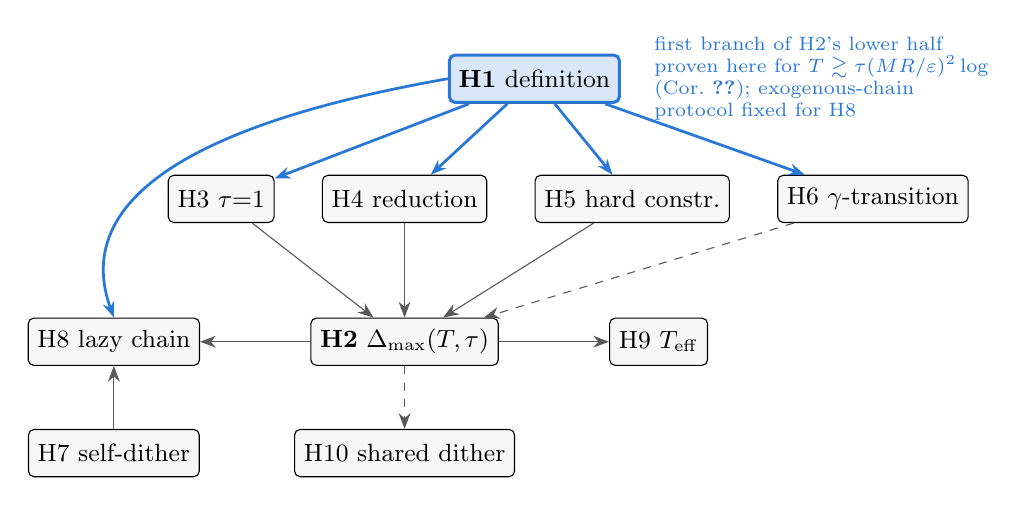
\begin{tikzpicture}[node distance=7mm and 9mm, every node/.style={font=\small},
  h/.style={draw,rounded corners=2pt,minimum width=12mm,minimum height=6mm,fill=gray!6},
  cur/.style={h,fill=hl!18,draw=hl,line width=1.1pt},
  ar/.style={-{Stealth[length=2mm]},gray!70!black}, dar/.style={ar,dashed}]
\node[cur] (H1) {\textbf{H1} definition};
\node[h,below left=9mm and 22mm of H1] (H3) {H3 $\tau{=}1$};
\node[h,right=6mm of H3] (H4) {H4 reduction};
\node[h,right=6mm of H4] (H5) {H5 hard constr.};
\node[h,right=6mm of H5] (H6) {H6 $\gamma$-transition};
\node[h,below=12mm of H4] (H2) {\textbf{H2} $\Dmax(T,\tau)$};
\node[h,right=14mm of H2] (H9) {H9 $T_{\rm eff}$};
\node[h,left=14mm of H2] (H8) {H8 lazy chain};
\node[h,below=8mm of H8] (H7) {H7 self-dither};
\node[h,below=8mm of H2] (H10) {H10 shared dither};
\draw[ar,line width=1pt,hl] (H1) -- (H3); \draw[ar,line width=1pt,hl] (H1) -- (H4);
\draw[ar,line width=1pt,hl] (H1) -- (H5); \draw[ar,line width=1pt,hl] (H1) -- (H6);
\draw[ar,line width=1pt,hl] (H1.west) to[out=190,in=110] (H8.north);
\draw[ar] (H3) -- (H2); \draw[ar] (H4) -- (H2); \draw[ar] (H5) -- (H2);
\draw[ar] (H2) -- (H8); \draw[ar] (H2) -- (H9); \draw[ar] (H7) -- (H8); \draw[dar] (H2) -- (H10); \draw[dar] (H6) -- (H2);
\node[font=\scriptsize,text=hl,align=left,right=3mm of H1] {first branch of H2's lower half\\proven here for $T\gtrsim\tau(MR/\varepsilon)^2\log$\\(Cor.~\ref{cor:lower}); exogenous-chain\\protocol fixed for H8};
\end{tikzpicture}
\caption{Dependencies between H1--H10 (arrows: ``is used by''). H1 (highlighted) supplies the definition used by all others; H3/H4 give the lower side of H2, H3/H5 the upper side; the rounding branch (H7, H8, H10) takes the transition point $\tau\approx T$ from H2.}
\label{fig:diagram}
\end{figure}

\textbf{Depends on:} nothing (H1 is the root). \textbf{Used by:} H2--H6 (the definition, the reduction of the class to $m$ and $\xi$), H8 (the protocol: the chain here is exogenous, a method-induced chain is excluded and must be handled separately), H9 (the proof below uses only uniform mixing, which is what H9 aims to weaken).

%=====================================================================================================
\section{Statement and motivation}\label{sec:statement}
\subsection{Setting and notation}
$\Ball=\{u\in\R^d:\norm u\le1\}$, $\Sph=\partial\Ball$, $e\sim\Unif(\Sph)$, $u\sim\Unif(\Ball)$, $B_r=r\Ball$; $d\ge2$.
For $g\in L^\infty(\R^d)$ the ball smoothing is $\hat g_\gamma(x)=\E_u g(x+\gamma u)=(g*\chi_\gamma)(x)$, $\chi_\gamma=\abs{B_\gamma}^{-1}\mathbf 1_{B_\gamma}$.
The ball and sphere multipliers are
\begin{equation}\label{eq:Psi}
\Psi_d(t)=\E_u e^{\mathrm i t u_1}=\Gamma(\tfrac d2+1)\big(\tfrac2t\big)^{d/2}J_{d/2}(t),\qquad
\Phi_d(t)=\E_e e^{\mathrm i t e_1}=\Gamma(\tfrac d2)\big(\tfrac2t\big)^{d/2-1}J_{d/2-1}(t),
\end{equation}
$\Psi_d(0)=\Phi_d(0)=1$; $j_{\nu,k}$ is the $k$-th positive zero of $J_\nu$. Fourier transform: $\hat u(\xi)=\int u(x)e^{-\mathrm i\ip\xi x}dx$ on $\cS'(\R^d)$.

\textbf{Oracle.} $O(x,s)=f(x)+\delta(x,s)$, $f$ convex and $M$-Lipschitz on $B_R$; $(s_k)$ is a Markov chain on a standard Borel space $(S,\mathcal S)$ with kernel $P$, stationary law $\pi$,
$d(t)=\sup_{s}\norm{P^t(s,\cdot)-\pi}_\TV$ and mixing time $\tau=\tmix=\min\{t\ge1:d(t)\le\frac14\}$.
$\delta:\R^d\times S\to[-\Delta,\Delta]$ is jointly Borel. The class condition of the problem statement is
\begin{equation}\label{eq:orth}
\E_{s\sim\pi}\E_e\big[\delta(x+\gamma e,s)\,e\big]=0\qquad\forall x. \tag{2}
\end{equation}
\textbf{Decomposition.} $m(x)=\E_\pi\delta(x,\cdot)$, $\xi=\delta-m$ (so $\abs m\le\Delta$, $\abs\xi\le2\Delta$, $\E_\pi\xi(x,\cdot)=0$ for every $x$).
\textbf{Bias at a fixed state} (two-point estimator $\hat g=\frac d{2\gamma}(O(x+\gamma e,s)-O(x-\gamma e,s))e$):
$b(x,s)=\frac d{2\gamma}\E_e[(\delta(x+\gamma e,s)-\delta(x-\gamma e,s))e]=\frac d\gamma\E_e[\delta(x+\gamma e,s)e]$ by $e\mapsto-e$.

\textbf{Two readings of (2)} for bounded measurable $\delta$: (A) for Lebesgue-a.e.\ $x$; (B) for every $x$.
\textbf{Regular class} $\cG_\gamma$: bounded Borel $g$ such that for every $x$ the set $\{\theta\in\Sph:\ g$ is discontinuous at $x+\gamma\theta\}$ has surface measure $0$.
Examples: continuous $g$; $g$ whose discontinuities lie on countably many affine hyperplanes (grid-cell hash noise, $\mathrm{sign}\sin\ip vx$ noise, rounding of a function affine on the stencil), because a hyperplane meets a sphere in a null set.

\subsection{Claims}
\begin{center}\small
\begin{tabularx}{\textwidth}{@{}lX@{}}
\toprule
H1.1 & $\frac d\gamma\E_e[\delta(x+\gamma e,s)e]=\nabla_x\hat\delta_\gamma(x,s)$ for a.e.\ $x$ (every $x$ in $\cG_\gamma$); $\E_\pi$ and $\E_e$ commute; (2) $\iff\hat m_\gamma\equiv{\rm const}$; the choice (A)/(B) does not change any result. \\
H1.2 & For fixed $\gamma$, $\Delta\cos(\ip\omega x+\varphi)$ is in the class iff $\gamma|\omega|\in\{j_{d/2,k}\}$; all admissible $m\in L^\infty$: $\widehat{m-c}$ is a single layer on the spheres $|\xi|=j_{d/2,k}/\gamma$. \\
H1.3 & (2) for all $\gamma\in(0,\gamma_0]$ $\Rightarrow m\equiv c$; stronger: two radii with $\gamma_1/\gamma_2\notin Q_d=\{j_{d/2,k}/j_{d/2,l}\}$ suffice; sharp. \\
H1.4 & Without a budget $\Dmax=\infty$: explicit algorithm with $\E\hat g=\nabla f_\gamma$ (up to an arbitrarily small bias), second moment $\lesssim dM^2+(d+\tau)d\Delta^2/\gamma^2$, and explicit $N(\Delta,\varepsilon,d,\tau)=O(\Delta^2)$. \\
H1.5 & Protocol variants and their effect on $\Dmax$; the complexity-preserving level $\Dcp=\Dmax(C\,T_0)$ is what the expected picture describes. \\
\bottomrule
\end{tabularx}
\end{center}

\subsection{Why it is worth checking; consequences}
If H1 holds, the two-sided bounds asked for in the problem statement are bounds on a \emph{function of the budget} $T$; the number $M\gamma/\sqrt d$ is the level up to which noise does not change the order of complexity, not a solvability boundary.
The class then splits cleanly: $m$ is a deterministic, radius-tuned part that is invisible at the method's radius; $\xi$ is a centred Markov part that costs only variance.
If H1 were false (e.g.\ if some bounded centred noise made $\varepsilon$ unattainable at any budget), the problem as stated would already have a finite answer and the expected picture would be a solvability boundary. The literal statement (``polynomial number of calls'') would then be meaningful.

%=====================================================================================================
\section{What is known}\label{sec:known}
\begin{center}\small
\begin{tabularx}{\textwidth}{@{}p{3.3cm}Xp{2.6cm}@{}}
\toprule
\textbf{Item} & \textbf{Statement as used here} & \textbf{Status here}\\\midrule
Ball smoothing gradient & $\nabla\hat f_\gamma(x)=\frac d\gamma\E_e[f(x+\gamma e)e]$; Flaxman, Kalai, McMahan (SODA 2005), Lemma~1, for integrable $f$ via Stokes; survey Gasnikov et al.\ arXiv:2211.13566, \S4.4 for condition (2) (theorem number in the survey not re-checked). & re-proved for $L^\infty$ with the a.e./everywhere distinction (Lemma~\ref{lem:stokes}) \\
Two-point second moment & $\E\norm{\hat g}^2\le c\,dM^2$, Shamir (JMLR 18, 2017), via concentration on the sphere. & re-derived with $c=d/(d-1)$ via Poincaré on $\Sph$ (Lemma~\ref{lem:var}) \\
MALN & Pasechnyuk-Vilensky, Pavlov, Takáč, Gasnikov, arXiv:2306.16371\textbf{v5}: Def.~II.1 (oracle $O_\delta(f)$, $T$ queries in $B_R$, randomized adaptive algorithm), Def.~II.2 ($(\varepsilon,\beta,\delta,T)$-solvability, $\Delta_\cF(\varepsilon,\beta,T)=\sup\{\delta\}$), Thm.~III.1 ($\Delta\le\frac43\varepsilon\theta^2+\frac53\frac{\varepsilon^2\theta}{MR}$, $\theta_*=\sqrt{2\ell/(n-1)}$, $\ell=\log\frac{2(T+1)}{1-\beta}$), Prop.~IV.1 (two-point method tolerates $\varepsilon^2/(84\sqrt nMR)$ for budgets $T\ge J(2K+1)$, $K=\lceil1200\,n^2M^2R^2/\varepsilon^2\rceil$, $J$ as defined there), Cor.~IV.4. The noise there is a fixed deterministic perturbation of $f$. & used as the template of Def.~\ref{def:dmax}; not re-proved \\
Pompeiu / mean-periodic & Schwartz (Ann.\ Math.\ 48, 1947): spectral synthesis for mean-periodic functions on $\R$. Brown, Schreiber, Taylor (Ann.\ Inst.\ Fourier 23(3), 1973, 125--154): Thm.~3.1/3.4 --- closed translation- and rotation-invariant subspaces of $C(\R^2)$ (remark: $\R^n$) are spanned by their exponential polynomials; Thm.~4.4 --- two discs of radii $r_1,r_2$ have the Pompeiu property iff $r_1/r_2\notin Q_1(0)$, a countable set defined by Bessel zeros (this two-disc Pompeiu theorem is also proved by Zalcman, Arch.\ Rational Mech.\ Anal.\ 47, 1972, 237--254); Thm.~4.7 is the area-measure version of Delsarte's two-radius \emph{harmonicity} theorem, taken from Zalcman [19] (a different statement, not used here). General $d$ and local versions: Berenstein--Zalcman (1976, 1980), Berenstein--Gay (Israel J.\ Math.\ 1986, $d=2$, requires $R>r_1+r_2$), Volchkov, \emph{Integral Geometry and Convolution Equations} (Kluwer 2003). & global statements re-proved for bounded $m$ by a tempered-distribution argument (Thm.~\ref{thm:fourier}, \ref{thm:tworadii}); the local and general-$d$ citations are \textbf{not re-checked} \\
Structure of distributions on a submanifold & Hörmander, \emph{ALPDO I}, Thm.~2.3.5: a distribution supported in $\{x''=0\}$ is locally $\sum_{|\alpha|\le k}u_\alpha\otimes\delta^{(\alpha)}(x'')$. & used \\
Mixing & $\bar d(s+t)\le\bar d(s)\bar d(t)$, $d\le\bar d\le2d$ $\Rightarrow d(\ell\tmix)\le2^{-\ell}$ (Levin--Peres--Wilmer, \emph{Markov Chains and Mixing Times}, Ch.~4). & used; numerically checked (V6) \\
Markov ZO & Prokhorov, Chebykin, Gasnikov, Beznosikov, arXiv:2601.01160: for gradient-free methods with Markov noise the cost of correlation is additive, $d+\tau$. & not used in proofs; consistent with Lemma~\ref{lem:var} \\
\midrule
Obtained earlier in this project & A pilot Monte Carlo run made before this study: $d=5$, $\gamma|\omega|=5.763$ gives $2.3\cdot10^{-4}$ at MC error $2.2\cdot10^{-4}$. Rounding with a uniform offset $c$ satisfies (2) for all radii under the uniform offset law: $\E_c\delta(x,c)$ is the mean of the rounding sawtooth over one period, a constant independent of $x$. & pilot: not re-checked as such (its value is reproduced in E1.1); rounding: direct argument \\
\midrule
New in this report & Lemma~\ref{lem:stokes}--Cor.~\ref{cor:cp}, Prop.~\ref{prop:wait}, Prop.~\ref{prop:q1}, Prop.~\ref{prop:quant}; experiments E1.1--E1.4; checks V1--V10, S1--S7. & \\
\bottomrule
\end{tabularx}
\end{center}

%=====================================================================================================
\section{Theory}\label{sec:theory}
\subsection{H1.1: bias at a fixed state, the two readings, and the reduction to $m$}

\begin{lemma}[Measurability and the swap]\label{lem:fubini}
Let $\delta:\R^d\times S\to[-\Delta,\Delta]$ be $\mathcal B(\R^d)\otimes\mathcal S$-measurable. Then $m=\E_\pi\delta(\cdot,s)$ is Borel, $\abs m\le\Delta$, and for \emph{every} $x$ and $\gamma>0$
\[\E_{s\sim\pi}\E_e[\delta(x+\gamma e,s)e]=\E_e\E_{s\sim\pi}[\delta(x+\gamma e,s)e]=\E_e[m(x+\gamma e)e].\]
\end{lemma}
\begin{proof}
The map $(\theta,s)\mapsto\delta(x+\gamma\theta,s)\theta_i$ is measurable on $\Sph\times S$ and bounded by $\Delta$, hence integrable for $\sigma\otimes\pi$; Fubini--Tonelli gives both the equality of the iterated integrals and the measurability of $m$.
\end{proof}
\begin{remark}
Joint measurability cannot be dropped: with separately measurable but not jointly measurable integrands the two iterated integrals may differ (Sierpiński-type examples). It is a natural assumption: $\delta$ is a function of $(x,s)$ computed by the oracle.
\end{remark}

\emph{Why Lemma~\ref{lem:stokes} should hold and where the difficulty is.} For smooth $g$ the identity is the divergence theorem on the ball. For $g\in L^\infty$ the right-hand side is a surface integral over the sphere $x+\gamma\Sph$, a Lebesgue-null set, so it depends on the representative of $g$; the left-hand side does not. The resolution: the spherical mean is defined for every $x$ for a given Borel function, but only its a.e.\ class is intrinsic.

\begin{lemma}[Ball Stokes identity for bounded functions]\label{lem:stokes}
Let $g$ be bounded Borel, $\gamma>0$, and $S_g(x)=\frac d\gamma\E_e[g(x+\gamma e)e]$ (defined for every $x$).
\begin{enumerate}[label=(\alph*)]
\item $\hat g_\gamma$ is Lipschitz with constant $\sqrt d\norm g_\infty/\gamma$ and $\nabla\hat g_\gamma=S_g$ a.e. If $g=g'$ a.e., then $S_g=S_{g'}$ a.e.
\item If $g\in\cG_\gamma$, then $S_g$ is continuous, $\hat g_\gamma\in C^1$ and $\nabla\hat g_\gamma(x)=S_g(x)$ for every $x$.
\item Without (b) the identity can fail at individual points: for $g(y)=\mathbf 1\{\norm y=\gamma\}\,\mathrm{sign}\,y_1$ one has $\hat g_\gamma\equiv0$ but $S_g(0)=\frac d\gamma\E\abs{e_1}\,\mathbf e_1\ne0$.
\end{enumerate}
\end{lemma}
\begin{proof}
(a) \emph{Smooth case.} If $g\in C^1_b$, then $\partial_i\hat g_\gamma(x)=\abs{B_\gamma}^{-1}\int_{B_\gamma}\partial_ig(x+z)dz=\abs{B_\gamma}^{-1}\int_{\partial B_\gamma}g(x+z)\frac{z_i}\gamma dS(z)$ by the divergence theorem, and with $\abs{\partial B_\gamma}=\gamma^{d-1}d\abs{\Ball}$, $\abs{B_\gamma}=\gamma^d\abs\Ball$ this is $(S_g)_i(x)$.
\emph{Bound.} For a unit $v$, $\abs{\ip{S_g(x)}v}\le\frac d\gamma\norm g_\infty\E\abs{\ip ev}\le\frac d\gamma\norm g_\infty(\E\ip ev^2)^{1/2}=\frac{\sqrt d}\gamma\norm g_\infty$.
\emph{General case.} Let $g_k=g*\varphi_k$ with a standard mollifier; $\norm{g_k}_\infty\le\norm g_\infty$, $g_k\to g$ a.e.\ and in $L^1_{\rm loc}$. Then $\hat g_{k,\gamma}\to\hat g_\gamma$ pointwise (dominated convergence), and each $\hat g_{k,\gamma}$ is $\sqrt d\norm g_\infty/\gamma$-Lipschitz, so is $\hat g_\gamma$. For a compact $K$,
$\int_K\norm{S_{g_k}-S_g}dx\le\frac d\gamma\int_{\Sph}\int_K\abs{g_k(x+\gamma\theta)-g(x+\gamma\theta)}dx\,d\sigma(\theta)\to0$, so $S_{g_k}\to S_g$ in $L^1_{\rm loc}$. For a test function $\phi$:
$\int\hat g_\gamma\partial_i\phi=\lim\int\hat g_{k,\gamma}\partial_i\phi=-\lim\int(S_{g_k})_i\phi=-\int(S_g)_i\phi$. A Lipschitz function is differentiable a.e.\ (Rademacher) and its a.e.\ gradient is its distributional gradient; hence $\nabla\hat g_\gamma=S_g$ a.e.
If $g=g'$ off a null set $N$ (w.l.o.g.\ Borel), then $\int_{\R^d}\sigma\{\theta:x+\gamma\theta\in N\}dx=\int_{\Sph}\abs{N-\gamma\theta}d\sigma=0$, so $S_g=S_{g'}$ for a.e.\ $x$.

(b) If $x_n\to x$, then $g(x_n+\gamma\theta)\to g(x+\gamma\theta)$ for $\sigma$-a.e.\ $\theta$ (the exceptional $\theta$ are those where $g$ is discontinuous at $x+\gamma\theta$), so $S_g(x_n)\to S_g(x)$ by dominated convergence. For a Lipschitz $u$ with $\nabla u=S$ a.e.\ and $S$ continuous, $u(x+h)-u(x)=\int_0^1\ip{S(x+th)}h\,dt$ holds for a.e.\ $x$ (Fubini along lines) and both sides are continuous in $x$, hence it holds for all $x$; so $u\in C^1$ with $\nabla u=S$.

(c) $g\ne0$ only on the sphere $\partial B_\gamma$, a null set, so $\hat g_\gamma\equiv0$; at $x=0$ every point $\gamma e$ lies on that sphere and $S_g(0)=\frac d\gamma\E[\mathrm{sign}(e_1)e]=\frac d\gamma\E\abs{e_1}\mathbf e_1$. For $x\ne0$ the sphere $x+\gamma\Sph$ meets $\partial B_\gamma$ in a null set and $S_g(x)=0$. (Checked numerically: V7.)
\end{proof}

\begin{proposition}[Reduction to $m$]\label{prop:reduction}
Under Lemma~\ref{lem:fubini}:
\begin{enumerate}[label=(\alph*)]
\item $b(x,s)=\nabla_x\hat\delta_\gamma(x,s)$ for a.e.\ $x$ (every $x$ if $\delta(\cdot,s)\in\cG_\gamma$), and $\norm{b(x,s)}\le\sqrt d\Delta/\gamma$ for all $x,s$.
\item Reading (A) of (2) $\iff$ $\nabla\hat m_\gamma=0$ a.e.\ $\iff$ $\hat m_\gamma\equiv c$ for a constant $c$, $\abs c\le\Delta$. The last condition is defined pointwise, is continuous in $x$, and depends only on the a.e.-class of $m$.
\item Reading (B) $\Rightarrow$ reading (A); if $m\in\cG_\gamma$ they are equivalent.
\item $\xi=\delta-m$ is unconstrained by (2) beyond $\E_\pi\xi(x,\cdot)=0$ for every $x$, which holds by construction. Under (2), $\E_\pi b(x,\cdot)=\E_\pi\nabla\hat\xi_\gamma(x,\cdot)=0$ a.e.: the noise is biased at a fixed state, with bias the gradient of the smoothed centred part, and unbiased on average over $\pi$.
\end{enumerate}
\end{proposition}
\begin{proof}
(a) Lemma~\ref{lem:stokes} applied to $g=\delta(\cdot,s)$ and the bound of its proof. (b) By Lemma~\ref{lem:fubini}, (2) at $x$ reads $S_m(x)=0$, and by Lemma~\ref{lem:stokes}(a) $S_m=\nabla\hat m_\gamma$ a.e. A Lipschitz function on the connected set $\R^d$ with a.e.\ vanishing gradient is constant (apply the line-integral formula of (b) of Lemma~\ref{lem:stokes} for a.e.\ $x$ and use continuity). (c) Lemma~\ref{lem:stokes}(b). (d) By (b), $\hat m_\gamma\equiv c$, so $\nabla\hat m_\gamma=0$ and $\E_\pi b=\E_\pi\nabla\hat\delta_\gamma=\nabla\hat m_\gamma+\E_\pi\nabla\hat\xi_\gamma$ a.e.
\end{proof}

\paragraph{Which reading to use, and why it does not matter.}
Let $\cN_A\supseteq\cN_B$ be the two classes. (i) Every structural statement below (Thm.~\ref{thm:fourier}--\ref{thm:tworadii}) is about the a.e.-class of $m$ and holds verbatim for both. (ii) The algorithmic result (Thm.~\ref{thm:alg}) holds for $\cN_B$ with $\rho=0$ and for $\cN_A$ with an arbitrarily small random-centre radius $\rho>0$, at the price of replacing $2M\gamma$ by $2M(\gamma+\rho)$ in the smoothing error: the query centre $y=x+\rho w$, $w\sim\Unif(\Ball)$ independent, has a density given the past, so it avoids the null set where (2) fails with probability one. (iii) Hard instances planned in H3/H5 use noise in $\cG_\gamma$ (hash noise on grid cells, $\mathrm{sign}\sin$ noise), where $\cN_A=\cN_B$. Hence $\Dmax^A\le\Dmax^B$ and every bound proven in this report or planned in H3--H5 holds for both.
\textbf{Recommendation:} state (2) for a.e.\ $x\in B_{R-\gamma}$ (reading A; representative-independent), and mention that within $\cG_\gamma$ it is the pointwise condition.

\subsection{H1.2: all admissible $m$ for a fixed radius}
\emph{Why it should be true.} $\hat m_\gamma=m*\chi_\gamma$ is a convolution, so in Fourier variables $\widehat{\hat m_\gamma}=\Psi_d(\gamma|\xi|)\,\hat m$; ``constant'' means ``supported at $\xi=0$''. Hence $\hat m$ can live only at $0$ and on the zero set of $\Psi_d(\gamma|\cdot|)$, a family of spheres. The only subtle point is the transversal order of $\hat m$ on these spheres; it is fixed by the simplicity of the Bessel zeros.

\begin{lemma}[Zeros of the multiplier]\label{lem:zeros}
$\Psi_d$ is an even entire function with $\Psi_d(0)=1$; its positive zeros are exactly $j_{d/2,k}$, all simple; $\psi_\gamma(\xi):=\Psi_d(\gamma|\xi|)$ is $C^\infty$ with all derivatives polynomially bounded, and $\nabla\psi_\gamma\ne0$ on $Z_\gamma:=\{\psi_\gamma=0\}=\bigcup_{k\ge1}\{|\xi|=r_k\}$, $r_k=j_{d/2,k}/\gamma$.
\end{lemma}
\begin{proof}
$\Psi_d(t)=\Gamma(\nu+1)\sum_{n\ge0}\frac{(-1)^n(t/2)^{2n}}{n!\,\Gamma(n+\nu+1)}$ with $\nu=d/2$, an even entire function; it is the Fourier transform of the uniform law on $\Ball$, so $\psi_\gamma$ is smooth with bounded derivatives. $\Psi_d'(t)=-\Gamma(\nu+1)2^\nu t^{-\nu}J_{\nu+1}(t)$ (from $(t^{-\nu}J_\nu)'=-t^{-\nu}J_{\nu+1}$; checked symbolically, S1). If $J_\nu(j)=J_{\nu+1}(j)=0$ then by $J_{\nu+1}=\frac\nu tJ_\nu-J_\nu'$ also $J'_\nu(j)=0$, and $J_\nu\equiv0$ by uniqueness for Bessel's ODE at $j>0$; so the zeros are simple and $\Psi_d'(j_{\nu,k})\ne0$ (S4). The zeros of the non-trivial entire function $\Psi_d$ are isolated, so $Z_\gamma$ is a locally finite union of spheres on which $\nabla\psi_\gamma=\gamma\Psi_d'(\gamma|\xi|)\xi/|\xi|\neq0$.
\end{proof}

\begin{theorem}[Fourier description of the fixed-radius class]\label{thm:fourier}
Let $m\in L^\infty(\R^d)$, $\gamma>0$, $c\in\R$. The following are equivalent:
\begin{enumerate}[label=(\roman*)]
\item $\hat m_\gamma\equiv c$ (i.e.\ (2) holds for a.e.\ $x$ with $\E_\pi\delta=m$);
\item $\psi_\gamma\cdot\widehat{(m-c)}=0$ in $\cS'(\R^d)$;
\item $\supp\widehat{(m-c)}\subset Z_\gamma$ and $\widehat{(m-c)}$ is a single layer on $Z_\gamma$: there are $T_k\in\mathcal D'(\{|\xi|=r_k\})$ with $\ip{\widehat{m-c}}\phi=\sum_k\ip{T_k}{\phi|_{|\xi|=r_k}}$ for all $\phi\in C_c^\infty$.
\end{enumerate}
The constant is unique: $\hat m$ coincides with $c(2\pi)^d\delta_0$ near $\xi=0$.
\end{theorem}
\begin{proof}
(i)$\iff$(ii). $\chi_\gamma$ has compact support, so $\widehat{m*\chi_\gamma}=\psi_\gamma\hat m$ for $m\in\cS'$ (exchange formula; Hörmander, \emph{ALPDO I}, Thm.~7.1.15 --- theorem number not re-checked). $\hat m_\gamma\equiv c\iff\psi_\gamma\hat m=c(2\pi)^d\delta_0\iff\psi_\gamma(\hat m-c(2\pi)^d\delta_0)=0$, since $\psi_\gamma\delta_0=\psi_\gamma(0)\delta_0=\delta_0$.
(ii)$\Rightarrow$(iii). Let $v=\widehat{m-c}$. If $\phi$ is supported in $\{\psi_\gamma\ne0\}$ then $\phi/\psi_\gamma\in C_c^\infty$ and $\ip v\phi=\ip{\psi_\gamma v}{\phi/\psi_\gamma}=0$; so $\supp v\subset Z_\gamma$. Near a point of $\{|\xi|=r_k\}$ use $y_1=\psi_\gamma(\xi)$ as the first coordinate of a local chart (Lemma~\ref{lem:zeros}: $\nabla\psi_\gamma\ne0$). By the structure theorem for distributions supported on a hyperplane (Hörmander, \emph{ALPDO I}, Thm.~2.3.5; number not re-checked), locally $v=\sum_{j\le J}v_j(y')\otimes\delta^{(j)}(y_1)$. Then $0=\psi_\gamma v=y_1v=\sum_{j\ge1}(-j)\,v_j\otimes\delta^{(j-1)}(y_1)$ (S6 checks $y_1\delta'=-\delta$), and uniqueness of the representation gives $v_j=0$ for $j\ge1$: $v=v_0\otimes\delta(y_1)$ is a single layer. A single layer in one chart is a single layer in any chart (the Jacobian is smooth and positive), so a partition of unity glues the local $v_0$ into $T_k\in\mathcal D'(\{|\xi|=r_k\})$.
(iii)$\Rightarrow$(ii). $\ip{\psi_\gamma v}\phi=\sum_k\ip{T_k}{(\psi_\gamma\phi)|_{|\xi|=r_k}}=0$ because $\psi_\gamma$ vanishes on each sphere.
Uniqueness of $c$: $v=\widehat{m-c}$ vanishes near $0$ by (iii), so near $0$, $\hat m=c(2\pi)^d\delta_0$.
\end{proof}
\noindent\textbf{Scope (global vs.\ local).} Thm.~\ref{thm:fourier} describes noises defined on all of $\R^d$ with (2) on all of $\R^d$. The class of Def.~\ref{def:dmax}(i) is local: $\delta$ need only be defined on $B_R$ and (2) is required for a.e.\ $x\in B_{R-\gamma}$. On $B_R$ the fixed-radius class is strictly larger, since local solutions of $m*\chi_\gamma=c$ need not extend to bounded solutions on $\R^d$. Restrictions to $B_R$ of the functions in Thm.~\ref{thm:fourier}(iii) are examples of the local class, and no full local description is claimed.

\begin{corollary}[Plane waves and examples]\label{cor:waves}
(a) For $m=\Delta\cos(\ip\omega x+\varphi)$, $\omega\ne0$: $\hat m_\gamma=\Psi_d(\gamma|\omega|)\,m$, hence $\E_e[m(x+\gamma e)e]=-\frac\gamma d\Delta\Psi_d(\gamma|\omega|)\sin(\ip\omega x+\varphi)\,\omega$, and $m$ is in the class iff $J_{d/2}(\gamma|\omega|)=0$.
(b) Any bounded superposition of such waves with frequencies on $\bigcup_k\{|\xi|=r_k\}$ is admissible; e.g.\ the radial Bessel function $x\mapsto\Phi_d(r_k|x|)$ ($T_k$ = surface measure; bounded by $1$, decays like $|x|^{-(d-1)/2}$). Each spherical component solves the Helmholtz equation $(\Delta_x+r_k^2)u=0$.
(c) For $d=1$, $j_{1/2,k}=k\pi$ and the class is exactly ``$m-c$ is $2\gamma$-periodic with zero mean'' (directly: $\int_{x-\gamma}^{x+\gamma}m=2\gamma c\ \forall x\Rightarrow m(x+\gamma)=m(x-\gamma)$ a.e.). For $d\ge2$ the ratios $j_{d/2,k}/j_{d/2,1}$ are not integers and admissible $m$ are not periodic in general.
(d) The first admissible frequency is $j_{d/2,1}/\gamma\approx(d/2+1.86(d/2)^{1/3})/\gamma$: $m$ oscillates on the scale $\gamma/d$.
\end{corollary}
\begin{proof}
(a) $\E_u\cos(a+\gamma\ip\omega u)=\mathrm{Re}\,e^{\mathrm ia}\E_ue^{\mathrm i\gamma\ip\omega u}=\Psi_d(\gamma|\omega|)\cos a$ since $\Psi_d$ is real; then Lemma~\ref{lem:stokes}(b) ($m$ is smooth). (b) Thm.~\ref{thm:fourier}(iii)$\Rightarrow$(i); $\widehat{\sigma_{r_k}}$ is $\Phi_d(r_k|x|)$ up to normalisation. (c),(d) as stated; the asymptotics of $j_{\nu,1}$ is classical (DLMF 10.21.40).
\end{proof}

\begin{remark}[Relation to mean-periodic functions]
Thm.~\ref{thm:fourier} is the \emph{tempered} (bounded) case, where the Fourier transform suffices. For general continuous solutions of $m*\chi_\gamma=c$ (not tempered) the description is by spectral synthesis: by Brown--Schreiber--Taylor (1973; Thm.~3.4 for $\R^2$, and a remark after Thm.~3.1 extending the ideal version to $\R^n$) the solution space, being closed and invariant under translations and rotations, is spanned by the exponential polynomials it contains, i.e.\ by $e^{\mathrm i\ip\zeta x}$ with $\zeta\in\mathbb C^d$, $\Psi_d(\gamma\sqrt{\zeta\cdot\zeta})=0$ (complex frequencies allowed). Boundedness removes the complex frequencies and leaves the real spheres of Thm.~\ref{thm:fourier}. We do not use the non-tempered theory.
\end{remark}

\begin{remark}[What the description does not say]
Thm.~\ref{thm:fourier} characterises admissible $m$ \emph{among bounded functions}. It does not characterise which single layers $\sum_kT_k$ have a bounded inverse Fourier transform (a hard problem, as is any intrinsic description of $\widehat{L^\infty}$). This is not needed below.
\end{remark}

\subsection{H1.3: several radii}
\emph{Why it should be true.} Each radius confines $\hat m$ to its own family of spheres; different families intersect only when a radius ratio equals a ratio of zeros, and a family of radii accumulating at $0$ leaves only $\xi=0$. For the ``all small radii'' version an even simpler argument works on a ball, without Fourier analysis.

\begin{theorem}[Radii accumulating at zero; local]\label{thm:allgamma}
Let $m\in L^\infty(B_R)$ and $\gamma_n\downarrow0$ with $\hat m_{\gamma_n}\equiv c_n$ on $B_{R-\gamma_n}$. Then $c_n\to c$ and $m=c$ a.e.\ on $B_R$. In particular, (2) for all $\gamma\in(0,\gamma_0]$ (for a.e.\ $x\in B_{R-\gamma}$) forces $\E_\pi\delta(x,\cdot)=c$ for a.e.\ $x$.
\end{theorem}
\begin{proof}
At every Lebesgue point $x$ of $m$ in the open ball, $x\in B_{R-\gamma_n}$ for large $n$ and $\hat m_{\gamma_n}(x)=c_n\to m(x)$ (Lebesgue differentiation). The limit is the same for all Lebesgue points because it is $\lim c_n$.
\end{proof}

\begin{theorem}[Two radii; global]\label{thm:tworadii}
Let $m\in L^\infty(\R^d)$ with $\hat m_{\gamma_1}\equiv c_1$ and $\hat m_{\gamma_2}\equiv c_2$ on $\R^d$. If $\gamma_1/\gamma_2\notin Q_d:=\{j_{d/2,k}/j_{d/2,l}:k,l\ge1\}$, then $c_1=c_2=:c$ and $m=c$ a.e. If $\gamma_1/\gamma_2=j_{d/2,k}/j_{d/2,l}$, the bounded smooth non-constant $m=\cos\ip\omega x$ with $|\omega|=j_{d/2,k}/\gamma_1=j_{d/2,l}/\gamma_2$ satisfies both conditions with $c_1=c_2=0$. $Q_d$ is countable (dense in $(0,\infty)$), so two radii in general position suffice.
\end{theorem}
\begin{proof}
Let $v=\hat m-c_1(2\pi)^d\delta_0$. By Thm.~\ref{thm:fourier} for $\gamma_1$, $\supp v\subset Z_{\gamma_1}\not\ni0$. Also $\psi_{\gamma_2}\hat m=c_2(2\pi)^d\delta_0$, so $\psi_{\gamma_2}v=(c_2-c_1)(2\pi)^d\delta_0$. The left side is supported in $Z_{\gamma_1}$, the right side in $\{0\}$; hence both vanish: $c_1=c_2$ and $\psi_{\gamma_2}v=0$, so $\supp v\subset Z_{\gamma_1}\cap Z_{\gamma_2}$. A common sphere means $j_{d/2,k}/\gamma_1=j_{d/2,l}/\gamma_2$, i.e.\ $\gamma_1/\gamma_2\in Q_d$; otherwise $Z_{\gamma_1}\cap Z_{\gamma_2}=\emptyset$, $v=0$, and $m=c_1$ a.e.\ by injectivity of the Fourier transform on $\cS'$. The converse is Cor.~\ref{cor:waves}(a). Density of $Q_d$: $j_{\nu,k}=(k+\frac\nu2-\frac14)\pi+O(1/k)$, so the ratios approximate all positive rationals.
\end{proof}

\begin{remark}[Regularity and the local version]
No regularity beyond boundedness and measurability is needed in Thms.~\ref{thm:fourier}--\ref{thm:tworadii}; the conclusion is $m=c$ \emph{a.e.}, which is all an oracle can be asked for (Lemma~\ref{lem:stokes}(c)). On a ball $B_R$ (the actual domain of the problem) Thm.~\ref{thm:allgamma} is proven above, while the two-radius statement needs a \emph{local} two-radius theorem; for $d=2$ this is Berenstein--Gay (1986) under $R>\gamma_1+\gamma_2$, and Volchkov (2003) treats general $d$. \textbf{We cite these without re-checking}; in the problem $R\gg\gamma_1+\gamma_2$, so the hypothesis of these theorems is satisfied.
\end{remark}

\emph{Quantitative caveat (new).} Qualitatively two radii suffice; quantitatively, a wave tuned to $\gamma_1$ is \emph{almost} admissible at every radius above roughly $\gamma_1\sqrt{2(d+2)}/j_{d/2,1}\approx2.8\gamma_1/\sqrt d$, because $\Psi_d$ decays like a Gaussian before its first zero and is exponentially small after it.
\begin{proposition}[Bias of a tuned wave at another radius]\label{prop:quant}
For $m=\Delta\cos(\ip\omega x+\varphi)$ and any $\gamma'>0$ the bias of the two-point estimator at radius $\gamma'$ (fixed state, averaged over $\pi$) is $\beta(\gamma')=\nabla\hat m_{\gamma'}(x)=-\Delta\Psi_d(\gamma'|\omega|)\sin(\ip\omega x+\varphi)\,\omega$, so $\sup_x\norm{\beta(\gamma')}=\Delta|\omega|\abs{\Psi_d(\gamma'|\omega|)}$. Moreover $\abs{\Psi_d(t)}\le\min\{1,\Gamma(\frac d2+1)(2/t)^{d/2}\}$, and for $|\omega|\ge j_{d/2,1}/\gamma$, $\gamma'\ge\gamma$:
$\sup_x\norm{\beta(\gamma')}\le\Delta|\omega|\,e\sqrt{d/2}\,(2/e)^{d/2}$ (for $d\ge2$).
\end{proposition}
\begin{proof}
The formula is Cor.~\ref{cor:waves}(a) with $\gamma'$. $\abs{J_\nu(t)}\le1$ for $\nu\ge0$, $t\in\R$ (DLMF 10.14.1) gives the bound on $\Psi_d$. For $t\ge j_{\nu,1}>\nu$ (DLMF 10.21.3) and Stirling's upper bound $\Gamma(\nu+1)\le e\,\nu^{\nu+1/2}e^{-\nu}$ ($\nu\ge1$): $\Gamma(\nu+1)(2/t)^\nu\le e\sqrt\nu(2/e)^\nu$.
\end{proof}
Numerically (E1.3), $\sup_{\gamma'\ge\gamma}\abs{\Psi_d(\gamma'j_{d/2,1}/\gamma)}=4.1\cdot10^{-2}$, $7.5\cdot10^{-4}$, $1.5\cdot10^{-10}$ for $d=5,20,100$, while at $\gamma'=0.1\gamma$ the tuned wave acts with most of its full bias $\Delta|\omega|\approx\Delta d/(2\gamma)$ (a Lipschitz systematic error): $|\Psi_d(0.1\,j_{d/2,k})|=0.976,0.942,0.896$ ($d=5$), $0.953,0.925,0.895$ ($d=20$), $0.852,0.824,0.798$ ($d=100$) for $k=1,2,3$. At $\gamma'=0.2\gamma$ the fraction is already smaller in high dimension: $0.909,0.784,0.633$ ($d=5$), $0.825,0.731,0.637$ ($d=20$), $0.525,0.459,0.404$ ($d=100$). Consequence for the recommendation: if two radii are used, the second must be \emph{small}, $\gamma_2\lesssim\gamma_1/\sqrt d$; the clean choice is all radii in $(0,\gamma_0]$.

\subsection{H1.4: without a budget, $\Dmax=\infty$}
\emph{Why it should be true.} At the method's own radius, $m$ contributes nothing on average (Prop.~\ref{prop:reduction}) and $\xi$ is centred over $\pi$; averaging over many states at a fixed point kills the state-dependent bias at rate $\tau/B$ in second moment, as for any bounded function of an ergodic chain. Two difficulties: (i) the iterate depends on past states, so states used at step $k$ are not distributed as $\pi$ given the iterate; a burn-in of $\tau\log$ rounds makes this bias as small as needed; (ii) the variance must be additive in $d$ and $\tau$, which requires one fresh direction per state.

\noindent\textbf{Algorithm 1} (batched ZO-SGD with burn-in; parameters $N,B,t_0,\eta,\rho$). Let $R'=R-\gamma-\rho>0$, $x_1=0$. For $k=1,\dots,N$:
(1) let $t_0$ rounds pass (queries in them are discarded or not made);
(2) draw $w_k\sim\Unif(\Ball)$ and set $y_k=x_k+\rho w_k$;
(3) in each of the next $B$ rounds $j=1..B$ draw a fresh $e_j\sim\Unif(\Sph)$ and query $y_k\pm\gamma e_j$ (both points in the same round, $q=2$);
(4) $\bar g_k=\frac1B\sum_j\frac d{2\gamma}\big(O(y_k+\gamma e_j,s)-O(y_k-\gamma e_j,s)\big)e_j$ with the state $s$ of that round;
(5) $x_{k+1}=\mathrm{Proj}_{B_{R'}}(x_k-\eta\bar g_k)$.
Output $\bar x=\frac1N\sum_kx_k$. Rounds used: $T=N(t_0+B)$; queries $2NB$.

\begin{lemma}[Second moment of a batch]\label{lem:var}
Let $\mathcal F_k$ contain everything up to the round before step (1) of iteration $k$, and let $s_0$ be the state of that round. Fix $y=y_k$. Write $\bar g=\frac1B\sum_j(a_j+\zeta_j+b_j)+\nabla f_\gamma(y)$ with $a_j=g_f(e_j)-\nabla f_\gamma(y)$, $g_f(e)=\frac d{2\gamma}(f(y+\gamma e)-f(y-\gamma e))e$, $b_j=b(y,s_{t_0+j})$, and $\zeta_j$ the rest. Then:
\begin{enumerate}[label=(\alph*)]
\item $\E[g_f(e)]=\nabla f_\gamma(y)$ and $\E\norm{g_f(e)}^2\le\frac{d^2M^2}{d-1}$;
\item $\big\|\E[\bar g\mid\mathcal F_k,y]-\nabla f_\gamma(y)\big\|\le2\,d(t_0+1)\,\frac{\sqrt d\Delta}\gamma$, provided $\E_\pi b(y,\cdot)=0$;
\item $\E\big[\norm{\bar g-\nabla f_\gamma(y)}^2\mid\mathcal F_k,y\big]\le\frac VB$, \quad $V:=\frac{2d^2M^2}{d-1}+(2d+8\tau-3)\frac{d\Delta^2}{\gamma^2}$.
\end{enumerate}
For $f\equiv0$ (noise only) (c) holds with $V=(d+8\tau-3)d\Delta^2/\gamma^2$.
\end{lemma}
\begin{proof}
(a) The mean is the ball Stokes identity for the continuous $f$ (Lemma~\ref{lem:stokes}(b)) and $e\mapsto-e$. The function $h(e)=f(y+\gamma e)$ is $\gamma M$-Lipschitz on $\Sph$, so by the Poincaré inequality on $\Sph$ (spectral gap $d-1$) $\mathrm{Var}\,h\le\gamma^2M^2/(d-1)$. Since $h(e)$ and $h(-e)$ have the same law, $\E(h(e)-h(-e))^2\le2\E(h(e)-\E h)^2+2\E(h(-e)-\E h)^2=4\mathrm{Var}\,h$, so $\E\norm{g_f}^2=\frac{d^2}{4\gamma^2}\E(h(e)-h(-e))^2\le\frac{d^2M^2}{d-1}$ (V5).
(b) Given $\mathcal F_k$ and $y$, the law of $s_{t_0+j}$ is $P^{t_0+j}(s_0,\cdot)$, the $e_j$ are independent of the states, and $\E[a_j+\zeta_j\mid\text{states}]=0$. Hence the conditional bias is $\frac1B\sum_j\int b(y,\cdot)\,d(P^{t_0+j}(s_0,\cdot)-\pi)$, bounded by $2\,d(t_0+j)\sup_s\norm{b(y,s)}\le2d(t_0+1)\sqrt d\Delta/\gamma$ (Prop.~\ref{prop:reduction}(a)).
(c) Let $X_j=a_j+\zeta_j$. Given all states and $(e_l)_{l\ne j}$, $X_j$ has mean zero, so cross terms $\E\ip{X_j}{X_l}$, $\E\ip{X_j}{b_l}$ vanish and
$\E\norm{\bar g-\nabla f_\gamma}^2=\frac1{B^2}\sum_j\E\norm{X_j}^2+\E\norm{\tfrac1B\sum_jb_j}^2$.
First, $X_j=Y_j-\E[Y_j\mid s_{t_0+j}]$ for $Y_j=g_f(e_j)+n_j$, $n_j=\frac d{2\gamma}(\delta(y+\gamma e_j,\cdot)-\delta(y-\gamma e_j,\cdot))e_j$, $\norm{n_j}\le d\Delta/\gamma$; so $\E\norm{X_j}^2\le\E\norm{Y_j}^2\le2\frac{d^2M^2}{d-1}+2\frac{d^2\Delta^2}{\gamma^2}$.
Second, with $H=\sqrt d\Delta/\gamma$ and $j<l$: $\abs{\E\ip{b_j}{b_l}}=\abs{\E\ip{b_j}{\E[b_l\mid s_{t_0+j}]}}\le H\cdot2d(l-j)H$, because $\E_\pi b(y,\cdot)=0$. With $d(t)\le2^{-\lfloor t/\tau\rfloor}$ and $\sum_{t\ge1}2^{-\lfloor t/\tau\rfloor}=2\tau-1$ (S5, V6):
$\E\norm{\sum_jb_j}^2\le BH^2+4H^2\sum_{j<l}d(l-j)\le BH^2(1+4(2\tau-1))=(8\tau-3)BH^2$.
Summing: $\E\norm{\bar g-\nabla f_\gamma}^2\le\frac1B\big[\frac{2d^2M^2}{d-1}+\frac{2d^2\Delta^2}{\gamma^2}+(8\tau-3)\frac{d\Delta^2}{\gamma^2}\big]=\frac VB$. For $f\equiv0$, $a_j=0$ and $\E\norm{X_j}^2\le d^2\Delta^2/\gamma^2$.
\end{proof}

\begin{theorem}[Any noise level is admissible at a polynomial budget]\label{thm:alg}
Let $f$ be convex and $M$-Lipschitz on $B_R$, $0<\varepsilon\le MR$, $\delta\in\cN(\Delta,\tau,\gamma)$ with (2) in reading (B), or in reading (A) and $\rho>0$, and $2M(\gamma+\rho)\le\varepsilon/2$, $\gamma+\rho<R$. Run Algorithm~1 with
\[
B=\Big\lceil\frac V{M^2}\Big\rceil,\quad N=\Big\lceil\frac{145}{4}\frac{M^2R^2}{\varepsilon^2}\Big\rceil,\quad \eta=\frac R{G\sqrt N},\ G=\sqrt{\tfrac{145}{64}}\,M,\quad
t_0=\tau\Big\lceil\log_2\frac{16R\sqrt d\,\Delta}{\gamma\varepsilon}\Big\rceil_+
\]
($t_0=0$ is allowed if $d(1)=0$, e.g.\ i.i.d.\ states). Then $\E f(\bar x)-f^*\le\varepsilon$ after
\begin{equation}\label{eq:T}
T(\Delta)=\Big\lceil\frac{145}{4}\frac{M^2R^2}{\varepsilon^2}\Big\rceil\left(\Big\lceil\frac{2d^2}{d-1}+(2d+8\tau-3)\frac{d\Delta^2}{M^2\gamma^2}\Big\rceil+\tau\Big\lceil\log_2\frac{16R\sqrt d\,\Delta}{\gamma\varepsilon}\Big\rceil_+\right)
\end{equation}
rounds ($2NB$ queries). The same holds for any initial law of the chain.
\end{theorem}
\begin{proof}
Let $F(x)=\E_wf_\gamma(x+\rho w)=\E f(x+\gamma u+\rho w)$; $F$ is convex and $M$-Lipschitz on $B_{R'}$, $f\le F\le f+M(\gamma+\rho)$ (Jensen and Lipschitz), and $\nabla F(x)=\E_w\nabla f_\gamma(x+\rho w)$ ($f_\gamma\in C^1$, Lemma~\ref{lem:stokes}(b)).
\emph{Bias.} The law of $y_k$ given $\mathcal F_k$ has a density, so $\E_\pi b(y_k,\cdot)=0$ a.s.\ in reading (A); in (B) it holds for every $y$. By Lemma~\ref{lem:var}(b) and $d(t_0+1)\le d(t_0)\le2^{-\lfloor t_0/\tau\rfloor}$: $\E[\bar g_k\mid\mathcal F_k]=\nabla F(x_k)+\beta_k$, $\norm{\beta_k}\le\beta:=\frac{\varepsilon}{8R}$.
\emph{Second moment.} $\E[\norm{\bar g_k}^2\mid\mathcal F_k,y_k]\le(\norm{\nabla f_\gamma(y_k)}+\beta)^2+\frac VB\le(M+\tfrac M8)^2+M^2=\tfrac{145}{64}M^2=G^2$ (using $\varepsilon\le MR$).
\emph{SGD.} Let $x_*'=\mathrm{Proj}_{B_{R'}}x_*$; $\norm{x_*-x_*'}\le\gamma+\rho$. Non-expansiveness of the projection gives
$\norm{x_{k+1}-x_*'}^2\le\norm{x_k-x_*'}^2-2\eta\ip{\bar g_k}{x_k-x_*'}+\eta^2\norm{\bar g_k}^2$; taking expectations, using convexity $\ip{\nabla F(x_k)}{x_k-x_*'}\ge F(x_k)-F(x_*')$ and $\abs{\ip{\beta_k}{x_k-x_*'}}\le2R\beta$, summing and dividing by $N$:
$\E F(\bar x)-F(x_*')\le\frac{R^2}{2\eta N}+\frac{\eta G^2}2+2R\beta=\frac{RG}{\sqrt N}+\frac\varepsilon4\le\frac\varepsilon2$ by the choice of $N$ ($16R^2G^2/\varepsilon^2=\frac{145}4M^2R^2/\varepsilon^2$, S5).
\emph{Back to $f$.} $f(\bar x)\le F(\bar x)$ and $F(x_*')\le f(x_*')+M(\gamma+\rho)\le f^*+2M(\gamma+\rho)\le f^*+\varepsilon/2$.
Rounds: $N(t_0+B)$, which is \eqref{eq:T}. The initial law enters only through $s_0$ in Lemma~\ref{lem:var}(b), which is uniform in $s_0$.
\end{proof}

\begin{corollary}[Degeneracy of the current definition; all-radii class, or fixed radius $\gamma\le\varepsilon/(4M)$]\label{cor:degenerate}
For every $\tau<\infty$, $\gamma\le\varepsilon/(4M)$ and every $\Delta<\infty$ the class is $\varepsilon$-solvable in expectation with $T(\Delta)$ rounds, $T(\Delta)\sim\frac{145}4(2d+8\tau-3)\frac{dR^2\Delta^2}{\gamma^2\varepsilon^2}$ as $\Delta\to\infty$ (V9 confirms slope $2.000$). Hence (i) $\Dmax=\infty$ if the budget is unrestricted; (ii) $\Dmax=\infty$ also under the literal ``polynomial number of calls'': for each fixed $\Delta$, $T(\Delta)$ is a polynomial in $(d,\tau,MR/\varepsilon,1/\gamma,\Delta)$; (iii) if instead the polynomial $p$ is fixed and independent of $\Delta$, the answer depends on $p$ (see Cor.~\ref{cor:lower}), so it is not a property of the class.
(iv) \emph{Scope.} In the all-radii class $\Gamma=(0,\gamma_0]$ of Def.~\ref{def:dmax} the conclusion holds without any condition on $\gamma_0$: by Thm.~\ref{thm:allgamma}, $m=c$ a.e.\ on $B_R$, so (2) holds at every radius (reading (A)), and Algorithm~1 runs at its own radius $\gamma'=\min\{\gamma_0,\varepsilon/(8M)\}$ with $\rho=\varepsilon/(8M)$. For the fixed-radius class with $\gamma>\varepsilon/(4M)$ \emph{nothing is proven}: a method must work at a smaller radius, where the Bessel part of $m$ acts as a systematic error (Prop.~\ref{prop:quant}, E1.3; hypothesis H6), and $\Dmax$ without a budget may be finite there.
(v) The statements are in the expectation variant; the probability variant follows by Cor.~\ref{cor:prob}.
\end{corollary}

\begin{corollary}[Budgeted lower bound; first branch of the lower half of H2]\label{cor:lower}
Let $\gamma\le\varepsilon/(4M)$ and $T_1(\Delta)=\frac{149}4\frac{M^2R^2}{\varepsilon^2}\big(\frac{2d^2}{d-1}+1+t_0(\Delta)\big)$. If $T\ge2T_1(\Delta)$ and
$\Delta\le\frac{\gamma\varepsilon}R\sqrt{\frac{T}{74.5\,(2d+8\tau-3)\,d}}$, then $\Delta$ is admissible with $T$ rounds in the expectation variant. Thus, up to the logarithm hidden in $t_0$ and for $T\ge2T_1$,
$\Dmax^{\E}(\varepsilon,d,\tau,\gamma;T)\ \gtrsim\ \frac{\varepsilon\gamma}R\sqrt{\frac T{d(d+\tau)}}$.
\end{corollary}
\begin{proof}
$N\le\frac{149}4M^2R^2/\varepsilon^2$ (since $MR/\varepsilon\ge1$) and $B\le V/M^2+1$, so $T(\Delta)\le\frac{149}4\frac{R^2}{\varepsilon^2}\big(V+M^2(1+t_0)\big)=T_1+\frac{149}4(2d+8\tau-3)\frac{dR^2\Delta^2}{\gamma^2\varepsilon^2}$; each part is $\le T/2$ under the assumptions. Algorithm~1 may idle the remaining rounds.
\end{proof}
\begin{remark}[What Cor.~\ref{cor:lower} does and does not give for H2]\label{rem:h2}
H2 conjectures
\[\Dmax\asymp\frac{\varepsilon\gamma}R\max\Big\{\sqrt{\frac T{d(d+\tau)}},\ \sqrt{\frac{\ln T}d}\Big\}\qquad(\gamma\le\gamma_\varepsilon),\]
including the regime $\tau\gtrsim T$.
(a) Cor.~\ref{cor:lower} proves only the \emph{first branch} of the lower half, and only for $\gamma\le\varepsilon/(4M)$ and $T\ge2T_1(\Delta)$. Since $T_1\ge\frac{149}4\frac{M^2R^2}{\varepsilon^2}t_0$ with $t_0=\tau\lceil\log_2(16R\sqrt d\Delta/(\gamma\varepsilon))\rceil_+$, this requires $T\gtrsim\tau(MR/\varepsilon)^2\log(R\sqrt d\Delta/(\gamma\varepsilon))$; the regime $\tau\gtrsim T$ is excluded by assumption.
(b) The \emph{second branch} $\frac{\varepsilon\gamma}R\sqrt{\ln T/d}$ is not addressed here. Without the factor $\sqrt{\ln T}$, it would follow from Prop.~IV.1 of Pasechnyuk-Vilensky et al.\ (arXiv:\allowbreak2306.16371v5) ($\varepsilon^2/(84\sqrt dMR)\ge\frac{\varepsilon\gamma}{84R\sqrt d}$ for $\gamma\le\varepsilon/M$, for budgets $T\ge J(2K+1)$, $K=\lceil1200\,d^2M^2R^2/\varepsilon^2\rceil$). This transfer needs the proof of Prop.~IV.1 to use only the per-query bound $|O-f|\le\Delta$. The noise in v5 is a \emph{fixed} perturbation of $f$, while a Markov noise returns different values at the same point, so it is not literally contained in the v5 class. \textbf{We have not re-checked this}; the second branch remains open here.
\end{remark}

\subsection{H1.5: the protocol, and the level that preserves complexity}
\begin{definition}[Protocol and $\Dmax$ --- proposed]\label{def:dmax}
Fix $d,R,M,\gamma\in(0,R)$, $\tau\ge1$, $q\ge1$, $\Gamma\subseteq(0,\gamma]$ (the set of radii in the class; $\Gamma=(0,\gamma]$ recommended, $\Gamma=\{\gamma\}$ the fixed-radius variant).
\begin{enumerate}[label=(\roman*)]
\item \emph{Noise instance:} a standard Borel $S$, a Markov kernel $P$ with stationary $\pi$ and $\tmix(P)\le\tau$, an arbitrary initial law, and a jointly Borel $\delta:\R^d\times S\to[-\Delta,\Delta]$ with $\E_\pi\E_e[\delta(x+\gamma'e,\cdot)e]=0$ for a.e.\ $x\in B_{R-\gamma'}$ and every $\gamma'\in\Gamma$. The class is $\cN_\Gamma(\Delta,\tau)$.
\item \emph{Protocol:} rounds $k=1,2,\dots$; the chain makes one step per round, $s_{k+1}\sim P(s_k,\cdot)$, independently of the algorithm (exogenous chain). In round $k$ the algorithm submits at most $q$ points of $B_R$, chosen measurably from its internal randomness and all previous answers, and receives $O(y,s_k)$ for each. \emph{Every round counts toward the budget, whether or not points are submitted.} After $T$ rounds it outputs $\hat x\in B_R$.
\item $\Dmax^{(q)}(\varepsilon,\beta;d,\tau,\Gamma;T)=\sup\big\{\Delta\ge0:$ there is an algorithm $A$ with $T$ rounds such that for all $f\in\cF^M_{\rm Lip}(B_R)$ and all instances in $\cN_\Gamma(\Delta,\tau)$, $\Prob\{f(\hat x)-\min f\le\varepsilon\}\ge1-\beta\big\}$, as in Def.~II.2 of v5. Expectation variant $\Dmax^{\E}$: $\E f(\hat x)-\min f\le\varepsilon$. The explicit bounds of this report (Thm.~\ref{thm:alg}, Cors.~\ref{cor:degenerate}--\ref{cor:cp}) are proven in the expectation variant; Cor.~\ref{cor:prob} transfers them to the probability variant with $\varepsilon\to\beta\varepsilon$.
\item \emph{Complexity-preserving level:} $\Dcp(C)=\Dmax(T=C\,T_0)$, $T_0=dM^2R^2/\varepsilon^2$.
\end{enumerate}
\end{definition}

\begin{proposition}[Free waiting removes $\tau$]\label{prop:wait}
Suppose idle rounds were free (only rounds with queries count). If an algorithm $A$ with $T$ query rounds $(\varepsilon,\beta)$-solves the class for i.i.d.\ states ($\tau=1$), then $A$ preceded in each round by $W=\tau\lceil\log_2(T/\eta)\rceil$ free idle rounds $(\varepsilon,\beta+\eta)$-solves the class for every chain with $\tmix\le\tau$. Consequently $\Dmax^{\rm free}(\varepsilon,\beta;{\rm iid};T)\ \ge\ \Dmax^{\rm free}(\varepsilon,\beta;\tau;T)\ \ge\ \Dmax^{\rm free}(\varepsilon,\beta-\eta;{\rm iid};T)$ for every $\eta\in(0,\beta)$: under free waiting the answer does not depend on $\tau$, except through an arbitrarily small loss in the confidence level. Here the argument ``iid'' denotes the class with i.i.d.\ states $s_k\sim\pi$ ($P(s,\cdot)=\pi$), \emph{not} the larger class $\tmix\le1$; the argument $\tau$ denotes the class $\tmix\le\tau$. The statement is for the probability variant; in the expectation variant the same argument changes $\E f(\hat x)-\min f$ by at most $\eta\cdot2MR$ (since $0\le f(\hat x)-\min f\le2MR$ on $B_R$).
\end{proposition}
\begin{proof}
The transcript is a measurable function of the algorithm's randomness, the directions and the states $(s_{r_1},\dots,s_{r_T})$ seen in query rounds. Given the past, the law of $s_{r_{i+1}}$ is $P^{W+1}(s_{r_i},\cdot)$, within $d(W)\le2^{-W/\tau}\le\eta/T$ of $\pi$ in total variation. A hybrid argument (replace the states one at a time by fresh $\pi$-draws) bounds the total-variation distance between the transcripts under the chain and under i.i.d.\ $\pi$ by $T\cdot\eta/T=\eta$, so the failure probability changes by at most $\eta$. The class with i.i.d.\ states is contained in the class with $\tmix\le\tau$ (an i.i.d.\ chain has $\tmix=1$), which gives the reverse inequality.
\end{proof}

\begin{proposition}[One query per state, $q=1$]\label{prop:q1}
If the chain advances with every query, Algorithm~1 with the two points of a pair in consecutive rounds is still unbiased up to $\beta$, with the state part of the second moment $\E\norm{\frac1B\sum_j\frac{b(y,s_{2j-1})+b(y,s_{2j})}2}^2\le\frac{(8\tau-3)d\Delta^2}{2B\gamma^2}$; Thm.~\ref{thm:alg} holds with $N(t_0+2B)$ rounds in place of $N(t_0+B)$. In particular $\Dmax=\infty$ without a budget also for $q=1$.
\end{proposition}
\begin{proof}
Given the states, $\E_e[\frac d{2\gamma}(\delta(y+\gamma e,s')-\delta(y-\gamma e,s''))e]=\frac12(b(y,s')+b(y,s''))$ by $e\mapsto-e$; the rest is Lemma~\ref{lem:var} applied to the $2B$ consecutive states. (V10 checks unbiasedness for $q=1$ and $q=2$.)
\end{proof}

\begin{corollary}[What the expected picture describes: the lower side]\label{cor:cp}
Let $\gamma\le\varepsilon/(4M)$ and $C\ge\frac{149}4\big(6+\frac{t_0}d\big)$ with $t_0=\tau\lceil\log_2\frac{16MR}{\varepsilon}\rceil$. Then, in the expectation variant, $\Dcp(C)\ge M\gamma/\sqrt{2d+8\tau-3}$. In particular, if $t_0=\tau\lceil\log_2(16MR/\varepsilon)\rceil\le d$ (the ceiling included), then $C=261=\lceil\frac{149}4\cdot7\rceil$ suffices and $\Dcp(261)\ge M\gamma/\sqrt{10d}$, which is the lower side of the ``expected picture'' $M\gamma/\sqrt d$ up to a constant. Without the ceiling, $\tau\log_2(16MR/\varepsilon)\le d$ gives only $t_0\le d+\tau$; since $\log_2(16MR/\varepsilon)\ge4$, this condition implies $\tau\le d/4$, and then $C=271$ is safe. For $\tau\gg d$ the required $C$ grows like $\tau\log(MR/\varepsilon)/d$, so ``complexity-preserving with an absolute constant $C$'' is \emph{not} what is proven in that regime.
\end{corollary}
\begin{proof}
For $\Delta\le M\gamma/\sqrt{2d+8\tau-3}$: $V/M^2\le\frac{2d^2}{d-1}+d\le5d$ ($d\ge2$) and $\frac{16R\sqrt d\Delta}{\gamma\varepsilon}\le\frac{16MR}\varepsilon$, so $T(\Delta)\le\frac{149}4\frac{M^2R^2}{\varepsilon^2}(5d+1+t_0)\le\frac{149}4\big(6+\frac{t_0}d\big)T_0\le C\,T_0$. For $C=271$: $t_0\le\tau(\log_2(16MR/\varepsilon)+1)\le d+\tau\le\frac54d$ (because $\tau\le d/\log_2(16MR/\varepsilon)\le d/4$), and $\frac{149}4(6+\frac54)=270.06$.
\end{proof}

\begin{corollary}[Probability variant]\label{cor:prob}
Let $\Dmax^{\E}(\varepsilon;T)$ and $\Dmax(\varepsilon,\beta;T)$ denote the expectation and the probability variants of Def.~\ref{def:dmax}(iii), with all other arguments equal. Then for every $\beta\in(0,1)$
\[\Dmax(\varepsilon,\beta;T)\ \ge\ \Dmax^{\E}(\beta\varepsilon;T).\]
Consequently, with all conditions of Thm.~\ref{thm:alg} and Cors.~\ref{cor:lower}, \ref{cor:cp} taken at accuracy $\beta\varepsilon$ (in particular $\gamma\le\beta\varepsilon/(4M)$, and $t_0,T_1$ evaluated at $\beta\varepsilon$):
(a) Thm.~\ref{thm:alg} run at accuracy $\beta\varepsilon$ gives $\Prob(f(\bar x)-f^*\le\varepsilon)\ge1-\beta$ after $T(\Delta)|_{\varepsilon\to\beta\varepsilon}$ rounds; the leading factor $\frac{145}4\frac{M^2R^2}{\varepsilon^2}$ becomes $\frac{145}4\frac{M^2R^2}{\beta^2\varepsilon^2}$, and $\Dmax=\infty$ without a budget also in the probability variant (same scope as Cor.~\ref{cor:degenerate});
(b) $\Dmax(\varepsilon,\beta;T)\ge\frac{\beta\varepsilon\gamma}R\sqrt{T/(74.5(2d+8\tau-3)d)}$ for $T\ge2T_1(\Delta)|_{\varepsilon\to\beta\varepsilon}$;
(c) $\Dmax(\varepsilon,\beta;C\,T_0/\beta^2)\ge M\gamma/\sqrt{2d+8\tau-3}$ for $C\ge\frac{149}4(6+t_0/d)$, $t_0=\tau\lceil\log_2\frac{16MR}{\beta\varepsilon}\rceil$, with $T_0=dM^2R^2/\varepsilon^2$; i.e.\ $\Dcp$ in the probability variant obeys the same lower bound with $C$ replaced by $C/\beta^2$.
\end{corollary}
\begin{proof}
If an algorithm gives $\E[f(\hat x)-\min f]\le\beta\varepsilon$, then, since $f(\hat x)-\min f\ge0$, Markov's inequality gives $\Prob(f(\hat x)-\min f>\varepsilon)\le\beta$. So every $\Delta$ admissible in the expectation variant at accuracy $\beta\varepsilon$ with $T$ rounds is admissible in the probability variant at $(\varepsilon,\beta)$ with $T$ rounds. (a)--(c) are Thm.~\ref{thm:alg}, Cor.~\ref{cor:lower} and Cor.~\ref{cor:cp} with $\varepsilon\to\beta\varepsilon$, using $T_0(\beta\varepsilon)=T_0(\varepsilon)/\beta^2$. A confidence-boosting step (independent restarts and a selection stage) would improve the dependence on $\beta$ to logarithmic; it is not needed for the conclusions of this report and is not carried out.
\end{proof}

\begin{remark}[Status of the matching upper bound]
That $\Dcp(C)\lesssim M\gamma/\sqrt d$ (for two-point methods of radius $\gamma$) is \textbf{not} proven here; it is the content of H3.2 (Assouad with rough noise). For arbitrary query points it may be false (H3.3, bandit methods).
\end{remark}

\paragraph{Protocol variants: effect on $\Dmax$.}
\begin{center}\small
\begin{tabularx}{\textwidth}{@{}p{3.3cm}p{4.0cm}Xp{1.9cm}@{}}
\toprule
\textbf{Variant} & \textbf{Effect on $\Dmax$ without budget} & \textbf{Effect on $\Dmax(T)$} & \textbf{Choice}\\\midrule
Chain step per call ($q=1$) vs per pair ($q=2$) & $\infty$ in both (Prop.~\ref{prop:q1}) & lower bound changes by a factor $\le2$ in $T$; upper bounds must be proven per $q$ & $q=2$, as in the statement \\
Free vs charged idle rounds & $\infty$ in both & free: $\tau$ disappears (Prop.~\ref{prop:wait}); charged: $\tau$ enters through $t_0$ and $8\tau$ in $V$ & charged \\
Arbitrary points vs stencil $x\pm\gamma e$ & $\infty$ in both (Alg.~1 uses the stencil) & arbitrary points can only increase $\Dmax(T)$ (inclusion of algorithm classes); for the fixed-radius class a different radius sees the Bessel part as systematic error (Prop.~\ref{prop:quant}); possible gain by bandit methods (H3.3) & arbitrary (information-theoretic), with $\Dmax^{\rm 2pt}$ reported separately \\
Repeating a point & cannot be forbidden ($x$ and $x+10^{-300}e$); useless within a round; across rounds it averages $\xi$ (H5.1) & no change: already included & allowed \\
Initial law: stationary vs arbitrary & $\infty$ in both & arbitrary costs nothing here (burn-in) & arbitrary \\
Exogenous vs method-induced chain & Alg.~1 needs exogenous & rounding (H8) violates exogeneity & exogenous; H8 separately \\
\bottomrule
\end{tabularx}
\end{center}

%=====================================================================================================
\section{Numerical verification}\label{sec:num}
All experiments use 5 seeds (fixed in the code), 95\% confidence intervals (Student-$t$ over seeds, or pooled standard errors where stated); every number below is computed from the stored raw results of the runs. Setups, predictions and refutation criteria of E1.1 and E1.2 were fixed in the formulation of the hypothesis before this study; for E1.3 and E1.4 they were written into the script headers before the runs. Theoretical curves are drawn on the same axes as the data. Symbolic and high-precision checks are listed in Appendix~\ref{app:checks}.

\subsection{E1.1: Monte Carlo for Bessel waves}
\textbf{Setup.} $m=\Delta\cos(\ip\omega x+\varphi)$, $\gamma=\Delta=1$, $d\in\{5,20,100\}$; w.l.o.g.\ $\omega=t\,\mathbf e_1$ (rotation invariance) and $\ip\omega x+\varphi=\pi/2$. (A) sweep: 60 values of $t=\gamma|\omega|$ including the first three zeros, $4\cdot10^5$ directions per seed (common across $t$); (B) at the zeros, random phase, $2\cdot10^6$ directions per seed, $\chi^2_d$ test of the whole vector against $0$; (C) superpositions of 10 waves with $|\omega_i|$ cycling over $j_{d/2,1..3}$, random directions and phases, amplitudes $\Delta/10$, tested at 20 random points per seed ($4\cdot10^5$ directions), plus a positive control with all frequencies detuned to $0.9\,j$.
\textbf{Prediction.} By Cor.~\ref{cor:waves}(a), $\ip{\E_e[m(x+\gamma e)e]}{\hat\omega}=-\Delta\,t\Psi_d(t)/d$ (this fixes the normalisation of the problem statement's ``$\Delta|\omega|\Psi_d(\gamma|\omega|)\gamma/d$'', with an extra factor $|\sin(\ip\omega x+\varphi)|$); zero at $t=j_{d/2,k}$.
\textbf{Refutation.} A non-zero mean at the zeros ($\chi^2$ rejection rate well above 5\%), or systematic deviation from the theory curve off the zeros.

\begin{figure}[h]\centering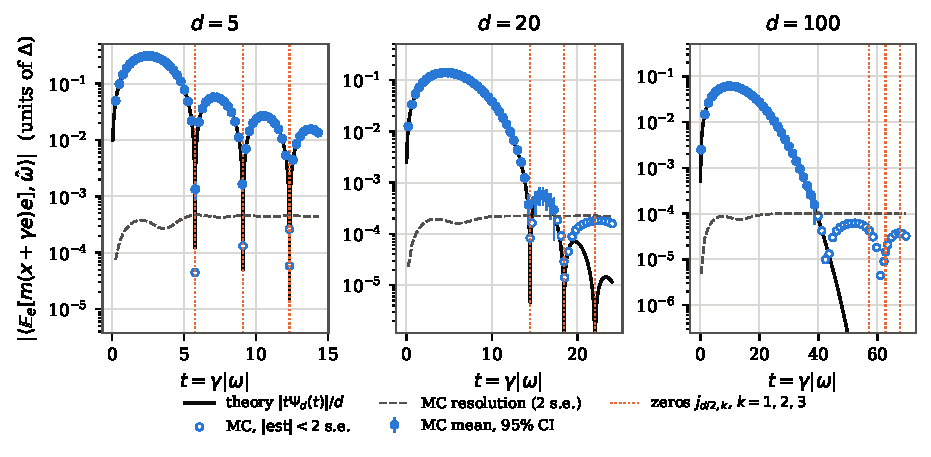
\includegraphics[width=\textwidth]{figs/e1_1_bessel_sweep.pdf}
\caption{E1.1, along-$\omega$ component of $\E_e[m(x+\gamma e)e]$ vs.\ $t=\gamma|\omega|$, log scale. Black: theory $|t\Psi_d(t)|/d$. Filled: MC mean over 5 seeds with 95\% CI; hollow: estimates within 2 s.e.\ of zero; dashed: MC resolution. In $d=100$ the signal falls below MC resolution already at $t\approx40$, long before the first zero $j_{50,1}=57.1$.}\label{fig:e11}
\end{figure}

\textbf{Result.} (A) Over 60 values of $t$ the standardised deviation from theory satisfies $\max|z|=0.64,\,1.87,\,1.24$ for $d=5,20,100$; no $|z|>2$ (the $z$'s are positively correlated across $t$ because of common random numbers). (B) At the zeros: $\chi^2_d$ $p$-values $\ge0.096,\,0.048,\,0.12$, rejections at 5\%: $0/15,\,1/15,\,0/15$; the ratio $\norm{\hat\E}/\sqrt{\sum{\rm se}_i^2}$ has median $0.92,\,0.96,\,1.00$ --- the estimate is exactly at the MC-noise level. The value of the pilot run of \S\ref{sec:known} ($d=5$, $2.3\cdot10^{-4}$ at error $2.2\cdot10^{-4}$) is reproduced. (C) Tuned superpositions: rejection of ``$\E[me]=0$'' in $4\%,\,2\%,\,7\%$ of 100 tests (nominal 5\%); detuned control: $100\%,\,93\%,\,11\%$. In $d=100$ the detuned signal has median norm $1.1\cdot10^{-8}$ against MC noise $3.5\cdot10^{-4}$, so MC has no power there; this regime is checked by 40-digit quadrature instead (S3: the identity $\E[\sin(te_1)e_1]=t\Psi_d(t)/d$ holds to relative accuracy $<10^{-20}$ at $0.95j$, $j$, $1.05j$ for the first three zeros, $d=100$).
\textbf{Verdict.} Prediction confirmed, normalisation confirmed. Observation: in high dimension the Bessel part is invisible to any sampling-based test long before the zeros --- relevant for H6.

\subsection{E1.2: logistic regression with rough noise, $\tau=1$}
\textbf{Setup.} $\ell_2$-regularised logistic regression as in the project's experiment on rounded oracles for convex problems (the same problem generator) with $d=10$, $n=50$, $\lambda=10^{-2}$; instance $=$ seed; domain $B_R$, $R=2\norm{x_*}$ ($\approx8.3$--$9.2$); $M=\norm A_{\rm op}/\sqrt n+\lambda R\approx0.54$; $\gamma=0.05$; $\Delta_{\rm ref}=M\gamma/\sqrt d$.
Noise: state $s=(k,\sigma)$, $k$ a fresh 64-bit key and $\sigma=\pm1$ drawn i.i.d.\ every round; $\delta(x,s)=\sigma\Delta\,\eta(\mathrm{hash}(\mathrm{cell}(x),k))$, $\eta=\pm1$, cubic cells of side $\gamma/(2\sqrt d)$. Then $m\equiv0$ (in the class for all radii) and the two values of a pair are independent $\pm\Delta$ --- the roughest admissible noise.
Method: Algorithm~1 with $t_0=0$, $N=300$, $\eta=0.5/L$, tail averaging over the last $N/2$ iterates (deviation from Thm.~\ref{thm:alg}, which averages all iterates; the problem is smooth and strongly convex, so the Lipschitz-class constants of the theorem are not used --- the experiment tests the \emph{scaling}). Grid: $\Delta\in\{0,1,10,100\}\Delta_{\rm ref}$, $B\in\{4^0,\dots,4^{b}\}$, $b=7,7,8,9$.
Control (outside the class): frozen state ($\tau=\infty$), noise $10\Delta_{\rm ref}\,\mathrm{sign}\sin(\sqrt d\ip vx/\gamma+\varphi)$, whose fixed-state bias $\asymp\sqrt d\Delta/\gamma$ cannot be averaged.
\textbf{Prediction} (fixed before the study): the target is reached for all $\Delta$, the required budget grows as $\Delta^2$. Made quantitative before the main run: primary target $\varepsilon=0.03$ ($\approx11\%$ of $f(0)-f^*$), per-seed $T_\varepsilon$ by log--log interpolation, slope over $\{10,100\}\Delta_{\rm ref}$ equal to $2\pm0.3$.
\textbf{Refutation.} An error floor independent of $T$ (as the control is expected to show).
\textbf{Deviation log.} The upper end of the $B$-grid for $100\Delta_{\rm ref}$ ($4^9$) was set after a timing pilot (seed 0, $B\le4096$, $10\Delta_{\rm ref}$) showed that $\varepsilon=0.03$ would not be reached with $B\le4^8$; $\varepsilon$ and the prediction were not changed. After the main run, the interpolation-free collapse test E1.2b was added (below), because the slope estimate depends on interpolation near the knee of the curves.

\begin{figure}[h]\centering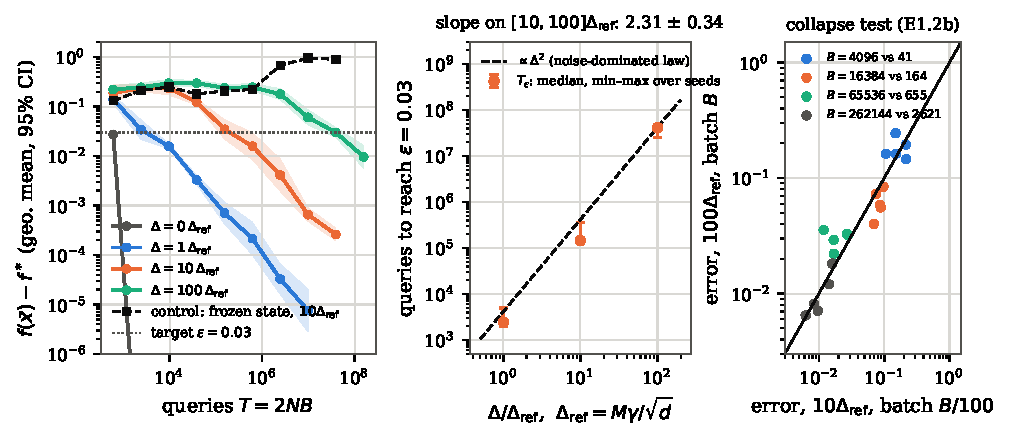
\includegraphics[width=\textwidth]{figs/e1_2_logistic.pdf}
\caption{E1.2. Left: $f(\bar x)-f^*$ vs.\ queries $T=2NB$ (log--log), geometric mean over 5 seeds with 95\% CI band; dashed black: frozen-state control. Middle: queries needed to reach $\varepsilon=0.03$ vs.\ $\Delta/\Delta_{\rm ref}$ (median, min--max over seeds), with the $\Delta^2$ law through the $100\Delta_{\rm ref}$ point. Right (E1.2b): error at $100\Delta_{\rm ref}$ with batch $B$ against error at $10\Delta_{\rm ref}$ with batch $B/100$, same seed; the diagonal is exact $\Delta^2$ scaling.}\label{fig:e12}
\end{figure}

\textbf{Result.} The target is reached in all $5/5$ seeds for every $\Delta$: median $T_\varepsilon=6.0\cdot10^2$ ($\Delta=0$, first grid point), $2.4\cdot10^3$ ($1\Delta_{\rm ref}$, range $1.9$--$5.0\cdot10^3$), $1.5\cdot10^5$ ($10\Delta_{\rm ref}$, $1.3$--$3.6\cdot10^5$), $4.2\cdot10^7$ ($100\Delta_{\rm ref}$, $2.5$--$4.6\cdot10^7$). At the largest batch the error at $100\Delta_{\rm ref}$ is still decreasing (median $8.2\cdot10^{-3}$ at $T=1.6\cdot10^8$): no floor. Slope of $\log T_\varepsilon$ in $\log\Delta$ on $[10,100]\Delta_{\rm ref}$ (paired per seed): $2.31\pm0.34$ (95\% CI $[1.97,2.65]$; per seed $2.37,2.55,2.47,2.31,1.84$); sensitivity to the target: $2.16\pm0.27$ ($\varepsilon=0.02$), $2.11\pm0.33$ ($0.05$), $2.03\pm0.15$ ($0.1$).
\textbf{E1.2b (collapse).} At matched batches ($B$ at $100\Delta_{\rm ref}$ vs.\ $B/100$ at $10\Delta_{\rm ref}$, 4 batch sizes $\times$ 5 seeds), $\log_{10}(\mathrm{err}_{100}/\mathrm{err}_{10})=0.017\pm0.081$, i.e.\ the error ratio is $1.04$ (95\% CI $[0.86,1.25]$): the error depends on $(\Delta,B)$ only through $B/\Delta^2$, within error.
\textbf{Control.} The frozen-state error does not decrease with $B$ (geometric mean $0.13\to0.90$ from $B=1$ to $4^8$; slope of the last four points $+0.33\pm0.59$): the refutation criterion has power.
\textbf{Verdict.} Qualitative prediction confirmed (the target is reached for every $\Delta$, no floor). The pre-registered quantitative criterion (slope $2\pm0.3$ at $\varepsilon=0.03$) is narrowly missed: the point estimate $2.31$ is $0.01$ above the band. Its CI $[1.97,2.65]$ contains $2$, the other targets give $2.03$--$2.16$, and the interpolation-free collapse test gives ratio $1.04$ $[0.86,1.25]$; we therefore report the budget law as ``consistent with $\Delta^2$'', not as a met pre-registered criterion. (H1.4b rests on the proof, not on E1.2.)

\subsection{E1.3: a tuned wave at a second radius}
\textbf{Setup.} $\gamma_1=\Delta=1$, $|\omega|=j_{d/2,k}$ ($k=1,2,3$), $d\in\{5,20,100\}$; 70 log-spaced ratios $\gamma_2/\gamma_1\in[0.05,3.2]$ plus all ratios of zeros in that range and $\sqrt2$; $10^6$ directions per seed. The quantity is the bias of the two-point estimator at radius $\gamma_2$, $\beta=(d/\gamma_2)\E_e[m(x+\gamma_2e)e]$, along $\hat\omega$ at $\sin=1$.
\textbf{Prediction.} $\abs\beta=\Delta|\omega|\abs{\Psi_d(\gamma_2|\omega|)}$ (Prop.~\ref{prop:quant}); zero exactly at $\gamma_2/\gamma_1=j_{d/2,l}/j_{d/2,k}$, non-zero at $\sqrt2$.
\textbf{Refutation.} Deviation from the curve beyond MC error; vanishing bias at a generic ratio.

\begin{figure}[h]\centering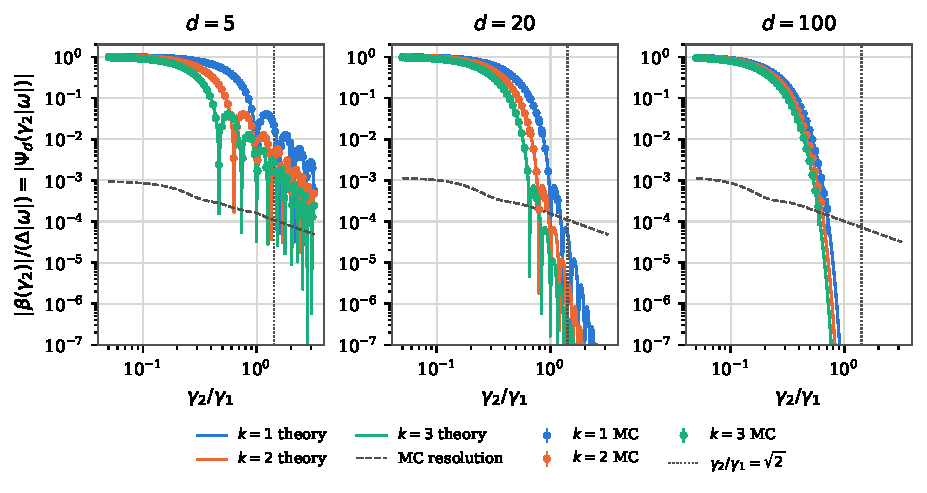
\includegraphics[width=\textwidth]{figs/e1_3_two_radii.pdf}
\caption{E1.3, normalised bias $|\beta(\gamma_2)|/(\Delta|\omega|)$ vs.\ $\gamma_2/\gamma_1$ (log--log) for waves tuned to the first three zeros at $\gamma_1$. Lines: $|\Psi_d(\gamma_2|\omega|)|$; dots: MC (5 seeds, 95\% CI), shown where resolved; dashed: MC resolution.}\label{fig:e13}
\end{figure}

\textbf{Result.} Over all resolved and unresolved points $\max|z|=1.14,\,2.41,\,1.85$; fraction $|z|>2$: $0\%,\,6.8\%,\,0\%$ of $276,\,309,\,315$ points (correlated through common random numbers). At $\gamma_2=\sqrt2\gamma_1$, $d=5$: measured $0.02232,\,0.00361,\,0.00270$ vs.\ theory $0.02231,\,0.00359,\,0.00270$ (s.e.\ $\le8.5\cdot10^{-5}$) --- a generic second radius detects the wave. For $d=20,100$ the theoretical value at $\sqrt2$ ($5\cdot10^{-5}$ and $3\cdot10^{-18}$) is below MC resolution. At $\gamma_2=0.1\gamma_1$ the theoretical bias (which the MC follows) is between $0.798\,\Delta|\omega|$ ($d=100$, $k=3$) and $0.976\,\Delta|\omega|$ ($d=5$, $k=1$), i.e.\ $\ge0.79\,\Delta|\omega|$ in all nine cases (values in Prop.~\ref{prop:quant} and in the stored results). Half-bias radius: $|\Psi_d|=\frac12$ at $\gamma_2/\gamma_1=0.52,\,0.38,\,0.21$ ($d=5,20,100$), matching $\sqrt{2\ln2\,(d+2)}/j_{d/2,1}$.
\textbf{Verdict.} Prediction confirmed. Refinement: a second radius kills a tuned wave in theory, but in practice only a \emph{smaller} radius $\gamma_2\lesssim\gamma_1\sqrt{2(d+2)}/j_{d/2,1}$ sees it with non-negligible bias.

\subsection{E1.4 (new): additivity of $d$ and $\tau$ in the batched second moment}
\textbf{Setup.} Noise $\delta(x,(k,\sigma))=\sigma\Delta\,\mathrm{sign}\sin(\sqrt d\ip{v_k}x/\gamma+\varphi_k)$, $K=512$ random $(v_k,\varphi_k)$, $\sigma=\pm1$ (so $\E_\pi\delta\equiv0$: in the class for all radii, maximal bias $\asymp\sqrt d\Delta/\gamma$ at a fixed state). Lazy resampling chain: stay with probability $\alpha=1-1/\tau_{\rm nom}$, else redraw from $\pi$; $\tau_{\rm nom}\in\{1,4,16,64,256\}$ ($\tmix=1,5,22,88,354$); $d\in\{10,40,160\}$; $f\equiv0$, $x=0$, $s_1\sim\pi$; $B=32\tmix+64$; 300 batches per seed.
\textbf{Prediction (exact, no free parameter).} $B\,\E\norm{\bar g}^2=A+S\,[1+2\sum_{t=1}^{B-1}(1-\frac tB)\alpha^t]$, where $S=\E_\pi\norm{b}^2$ and $A=\E\norm{n}^2-S$ are computed by exact one-dimensional integrals over the law of $e_1$ (incomplete beta function); this follows from the proof of Lemma~\ref{lem:var}(c) with the exact autocorrelation $\alpha^t$ of the lazy chain. Bound: $(d+8\tmix-3)\,d\Delta^2/\gamma^2$.
\textbf{Refutation.} Deviations beyond the pooled MC error; growth like $d\cdot\tau$.

\begin{figure}[h]\centering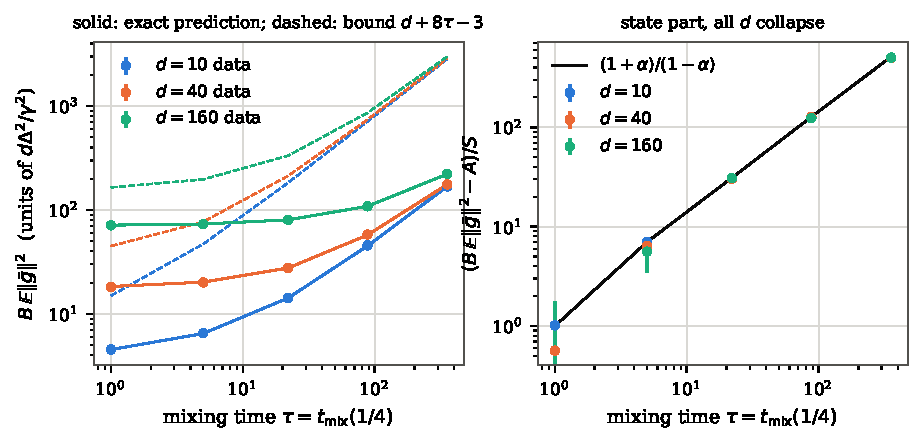
\includegraphics[width=0.95\textwidth]{figs/e1_4_batch_variance.pdf}
\caption{E1.4. Left: $B\E\norm{\bar g}^2$ in units of $d\Delta^2/\gamma^2$ vs.\ $\tmix$ (log--log); solid: exact prediction; dashed: bound of Lemma~\ref{lem:var}. Right: state part $(B\E\norm{\bar g}^2-A)/S$; all dimensions collapse onto $(1+\alpha)/(1-\alpha)$ (finite-$B$ version), slope 1 in $\tau$.}\label{fig:e14}
\end{figure}

\textbf{Result.} In all 15 cells the relative deviation from the exact prediction is $\le1.41\%$, pooled $z\in[-1.19,1.55]$. Slope of the state part vs.\ $\tmix$ (log--log, $\tmix\ge5$): $1.003\pm0.025$, $1.02\pm0.05$, $1.05\pm0.11$ for $d=10,40,160$. Fitted constants: $A/d^2=0.42$--$0.45$, $S/d=0.30$--$0.33$, so $B\E\norm{\bar g}^2\approx(0.44\,d+0.43\,\tmix)\,d\Delta^2/\gamma^2$ --- additive in $d$ and $\tau$, $\le0.43$ of the bound.
\textbf{Verdict.} Prediction confirmed; the constant $8$ of Lemma~\ref{lem:var} is conservative by a factor $\approx20$ for this chain.

%=====================================================================================================
\section{Verdict}\label{sec:verdict}
\begin{center}\small
\begin{tabularx}{\textwidth}{@{}p{5.2cm}p{3.0cm}X@{}}
\toprule
\textbf{Claim} & \textbf{Status} & \textbf{Support}\\\midrule
H1.1a $E_\pi$ and $E_e$ commute & proven under a condition (joint measurability) & Lemma~\ref{lem:fubini} \\
H1.1b $\frac d\gamma\E_e[\delta(x+\gamma e,s)e]=\nabla\hat\delta_\gamma$ & proven: a.e.\ for bounded Borel; everywhere in $\cG_\gamma$; fails pointwise otherwise & Lemma~\ref{lem:stokes}; V3 (smooth and rough, $\max|z|\le1.7$), V7 \\
H1.1c (2) $\iff\hat m_\gamma\equiv c$; $\xi$ unconstrained & proven & Prop.~\ref{prop:reduction} \\
H1.1d choice of reading does not affect results & proven for all results of this report; for H3/H5 under the condition that their constructions lie in $\cG_\gamma$ & \S\ref{sec:theory}, ``Which reading'' \\
H1.2a plane wave admissible iff $J_{d/2}(\gamma|\omega|)=0$; normalisation $\Delta t\Psi_d(t)/d$ & proven; confirmed numerically & Cor.~\ref{cor:waves}; E1.1; S2, S3 \\
H1.2b full description via single layers on spheres & proven on $\R^d$ (bounded $m$, global); on $B_R$ the class is larger, examples only & Thm.~\ref{thm:fourier}; S4, S6 \\
H1.3a all $\gamma\le\gamma_0$ (or $\gamma_n\to0$) $\Rightarrow m\equiv c$ & proven (local, on $B_R$) & Thm.~\ref{thm:allgamma} \\
H1.3b two radii with ratio $\notin Q_d$ suffice; sharp & proven on $\R^d$ for bounded measurable $m$; on $B_R$ only cited (local two-radius theorem) & Thm.~\ref{thm:tworadii}; V8; E1.3 \\
H1.3c a second radius $\gamma_2\gtrsim\gamma_1$ is quantitatively weak in high $d$ & proven for plane waves (bound), confirmed numerically & Prop.~\ref{prop:quant}; E1.3 \\
\bottomrule
\end{tabularx}
\end{center}
\begin{center}\small
\begin{tabularx}{\textwidth}{@{}p{5.2cm}p{3.0cm}X@{}}
\toprule
\textbf{Claim} & \textbf{Status} & \textbf{Support}\\\midrule
H1.4a explicit algorithm, bias $\le\varepsilon/(8R)$, second moment $\le V/B$, $V\asymp dM^2+(d+\tau)d\Delta^2/\gamma^2$ & proven & Lemma~\ref{lem:var}; E1.4 (exact to $1.41\%$); V5, V6, V10 \\
H1.4b $T(\Delta)=O(\Delta^2)$ explicit; $\Dmax=\infty$ without budget and under ``polynomial calls'' & proven under a condition: all-radii class (unconditional), or fixed-radius class with $\gamma\le\varepsilon/(4M)$; expectation variant, probability variant with $\varepsilon\to\beta\varepsilon$ & Thm.~\ref{thm:alg}, Cors.~\ref{cor:degenerate}, \ref{cor:prob}; V9; E1.2 \\
H1.4c $\Dmax(T)\gtrsim\frac{\varepsilon\gamma}R\sqrt{T/(d(d+\tau))}$ (first branch of H2's lower half) & proven under conditions: $\gamma\le\varepsilon/(4M)$, $T\ge2T_1(\Delta)$ (so $T\gtrsim\tau(MR/\varepsilon)^2\log$, not the regime $\tau\gtrsim T$), up to $\log$ in $t_0$ and constants; expectation variant, probability variant with $\varepsilon\to\beta\varepsilon$ & Cors.~\ref{cor:lower}, \ref{cor:prob}; Remark~\ref{rem:h2} \\
H1.5a free idle rounds make $\tau$ irrelevant & proven (probability variant; comparison with the i.i.d.\ class) & Prop.~\ref{prop:wait} \\
H1.5b $q=1$ vs $q=2$: same degeneracy & proven & Prop.~\ref{prop:q1}; V10 \\
H1.5c $\Dcp(C)\ge M\gamma/\sqrt{2d+8\tau-3}$ (the expected picture, lower side) & proven for $C\ge\frac{149}4(6+t_0/d)$ and $\gamma\le\varepsilon/(4M)$, expectation variant ($C=261$ if $\tau\lceil\log_2(16MR/\varepsilon)\rceil\le d$); probability variant with $\varepsilon\to\beta\varepsilon$, $C\to C/\beta^2$ & Cors.~\ref{cor:cp}, \ref{cor:prob} \\
H1.5d $\Dcp(C)\lesssim M\gamma/\sqrt d$ (upper side) & remains a hypothesis (H3.2) & --- \\
\bottomrule
\end{tabularx}
\end{center}

%=====================================================================================================
\section{Implications}\label{sec:contrib}
\subsection{For the general problem}
\begin{enumerate}
\item Without a budget the threshold degenerates: $\Dmax=\infty$ in the all-radii class (unconditionally) and in the fixed-radius class with $\gamma\le\varepsilon/(4M)$, also under ``polynomially many calls'' (Cor.~\ref{cor:degenerate}; proven under these conditions, expectation variant, probability variant by Cor.~\ref{cor:prob}). A non-degenerate threshold is therefore the \emph{function} $\Dmax(T)$ of the round budget, with the protocol fixed as in Def.~\ref{def:dmax}.
\item The ``expected picture'' is a statement about $\Dcp(C)=\Dmax(C\,T_0)$; its lower side is proven for $\gamma\le\varepsilon/(4M)$ and $C\ge\frac{149}4(6+t_0/d)$, in the expectation variant (Cor.~\ref{cor:cp}; probability variant by Cor.~\ref{cor:prob}); the upper side remains a hypothesis (H3.2).
\item The class: (2) for all radii in $(0,\gamma_0]$ is equivalent to $\E_\pi\delta(x,\cdot)={\rm const}$ for a.e.\ $x$ (Thm.~\ref{thm:allgamma}, proven). In this class $\gamma$ does not enter the class and is a parameter of the algorithm; the fixed-radius class contains Bessel waves (Thm.~\ref{thm:fourier}, proven), whose effect on other radii is H6.
\item Uniform geometric ergodicity enters only through $d(t)\le2^{-\lfloor t/\tau\rfloor}$ (Lemma~\ref{lem:var}); for a general state space this \emph{is} uniform ergodicity, so H1 does not weaken this assumption of the problem statement; weakening it is H9.
\item Rounding with a uniform offset satisfies (2) for all radii ($\E_c\delta$ is the period mean of the rounding sawtooth, a constant), i.e.\ it lies in the all-radii class with $m\equiv{\rm const}$. But the rounding chain is method-induced, which Def.~\ref{def:dmax} excludes; rounding is in $\cN$ only after the H8 extension.
\end{enumerate}

\subsection{For the other hypotheses}
H2: the \emph{first branch} of its lower half ($\gtrsim\frac{\varepsilon\gamma}R\sqrt{T/(d(d+\tau))}$) is proven up to the burn-in logarithm, for $\gamma\le\varepsilon/(4M)$ and $T\ge2T_1(\Delta)$, i.e.\ in the regime $T\gtrsim\tau(MR/\varepsilon)^2\log(R\sqrt d\Delta/(\gamma\varepsilon))$, in the expectation variant (Cor.~\ref{cor:lower}). Not covered: the regime $\tau\gtrsim T$, the second branch $\frac{\varepsilon\gamma}R\sqrt{\ln T/d}$ (Remark~\ref{rem:h2}: without $\sqrt{\ln T}$ and for $T\ge J(2K+1)$ it may follow from arXiv:2306.16371v5, Prop.~IV.1, not re-checked), and the whole upper half.
H4: the variance part of the reduction to Prokhorov et al.\ is done directly (Lemma~\ref{lem:var}); what remains for H4 is removing the burn-in $\log$ and last-iterate guarantees.
H3: the setting is now fixed (Def.~\ref{def:dmax}); the upper bound $\Dcp\lesssim M\gamma/\sqrt d$ is exactly H3.2.
H5.1: consistent (``repeat and average'' is another route to $\Dmax=\infty$).
H6: supported. Its mechanism --- for $\gamma>\gamma_\varepsilon$ the method must use a smaller radius, where the Bessel part of $m$ acts as a systematic error of size $\approx\Delta d/(2\gamma)$ --- is confirmed by Prop.~\ref{prop:quant} and E1.3 (bias $\ge0.79$--$0.98\,\Delta|\omega|$ at $\gamma_2=0.1\gamma_1$). What this report adds for H6 concerns only experiments that vary the radius: for such experiments the range $\gamma'>\gamma$ is uninformative for $d\ge20$ (bias $\le7.5\cdot10^{-4}\,\Delta|\omega|$, below Monte Carlo resolution). In the recommended all-radii class H6 does not arise.
H8, H9: the exogenous-chain assumption and the use of uniform mixing are now explicit; these are the two places to relax.

\subsection{Open questions}
\begin{itemize}
\item The upper side of the complexity-preserving level, $\Dcp(C)\lesssim M\gamma/\sqrt d$ for two-point methods of radius $\gamma$ (H3.2); for arbitrary query points it may be false (H3.3).
\item The second branch $\frac{\varepsilon\gamma}R\sqrt{\ln T/d}$ of the lower half of H2 and the regime $\tau\gtrsim T$ (Remark~\ref{rem:h2}).
\item The fixed-radius class with $\gamma>\varepsilon/(4M)$, where $\Dmax$ without a budget may be finite (Cor.~\ref{cor:degenerate}(iv); H6).
\item The two-radius theorem on a ball $B_R$ (only cited here) and the fixed-radius class on $B_R$, which is larger than on $\R^d$ (Thm.~\ref{thm:fourier} and the scope paragraph after it).
\item The modelling choices on which $\Dmax$ depends: whether idle rounds count (if they are free, $\tau$ drops out, Prop.~\ref{prop:wait}), whether the $q$ points of one state are arbitrary or only $x\pm\gamma e$ ($\Dmax$ vs.\ $\Dmax^{2\rm pt,\gamma}$), and whether (2) is required at one radius or at all radii $\le\gamma_0$. Def.~\ref{def:dmax} fixes one choice; \S\ref{sec:theory} (H1.5) lists the effect of the others.
\item A method-induced chain (H8) and mixing assumptions weaker than uniform ergodicity (H9).
\end{itemize}

\subsection{Scope of the novelty}
The problem statement already says ``polynomial number of calls'', and the MALN framework of Pasechnyuk-Vilensky et al.\ (arXiv:2306.16371v5, Def.~II.2) already carries $T$; if the complexity-preserving level is the intended object of the problem, then the definitional part of H1 is a clarification rather than a new result. What is new regardless: the structure theorem for the class (Thms.~\ref{thm:fourier}--\ref{thm:tworadii}, Prop.~\ref{prop:quant}), the explicit budget formula with additive $d+\tau$ and its corollary --- the first branch of the lower half of H2, in the regime $T\gtrsim\tau(MR/\varepsilon)^2\log$ --- and the protocol sensitivity (Prop.~\ref{prop:wait}).

%=====================================================================================================
\appendix
\section{Verification checks}\label{app:checks}
\begin{center}\small
\begin{tabularx}{\textwidth}{@{}lXl@{}}
\toprule
\textbf{ID} & \textbf{Check} & \textbf{Outcome}\\\midrule
V1 & $\Psi_d(t)=\E_u\cos(tu_1)$, quadrature, $d\in\{2,3,5,20\}$ & err $6\cdot10^{-15}$ \\
V2 & $\Phi_d'=-(t/d)\Psi_d$, finite differences, $d\le100$ & err $1.4\cdot10^{-9}$ \\
V3 & ball Stokes: MC sphere integral vs.\ finite differences of the ball mean ($d=5$; smooth waves and grid-hash noise) & $\max|z|=1.2$ (smooth), $1.7$ (rough); vs.\ exact $1.6$ \\
V4 & $\E|e_1|\le1/\sqrt d$; worst-case bias $\le\sqrt d\Delta/\gamma$ & pass \\
V5 & $\E\norm{g_f}^2\le d^2M^2/(d-1)$ for four test functions, $d\in\{2,5,20\}$ & max ratio $0.95$ \\
V6 & $\sum_{t\ge1}2^{-\lfloor t/\tau\rfloor}=2\tau-1$; $d(\ell\tmix)\le2^{-\ell}$; $\sum d(t)\le2\tmix-1$ (lazy chains) & pass \\
V7 & pointwise failure off $\cG_\gamma$ (Lemma~\ref{lem:stokes}(c)) & $S_g(0)_1=1.875=5\E|e_1|$, $0$ elsewhere \\
V8 & $\sqrt2,1.5,\pi/2\notin Q_5$; distance to $Q_5$ shrinks with the number of zeros & pass \\
V9 & formula~\eqref{eq:T}: slope of $\log T$ in $\log\Delta$ & $2.000$ \\
V10 & Algorithm~1 unbiased under a lazy chain, $q=2$ and $q=1$ & $\max|z|=1.6,\ 2.7$ ($d$ components) \\
S1 & $(t^{-\nu}J_\nu)'=-t^{-\nu}J_{\nu+1}$, $\Phi_d'=-(t/d)\Psi_d$ (sympy, general $d$) & exact \\
S2 & $\Psi_1,\Psi_3$ exact; $\Psi_2,\Psi_5$ to 50 digits & exact / $3\cdot10^{-51}$ \\
S3 & plane-wave identity at $d=100$ near the zeros, 40 digits & rel.\ err $<10^{-20}$ \\
S4 & simple zeros, $J_{d/2+1}(j_{d/2,k})\neq0$ & pass \\
S5 & constants $145/64$, $145/4$; block sum & exact \\
S6 & $\rho\,\delta'(\rho)=-\delta(\rho)$ & exact \\
S7 & $\E|e_1|$ formula $\le1/\sqrt d$, $d=2..200$ & pass \\
\bottomrule
\end{tabularx}
\end{center}
V1--V10 are numerical checks (numpy and scipy); S1--S7 are symbolic and high-precision checks (sympy and mpmath). All runs together take $\approx35$ min on 2 CPU cores (E1.2 dominates). Figures are built from the stored raw results only.

\paragraph{What was not checked.} The local two-radius theorem on a ball and the general-$d$ Pompeiu literature (cited only); the theorem number in the survey arXiv:2211.13566; the results of Prokhorov et al.\ (not used in proofs); experiments with $\tau>1$ on an optimisation problem (E1.4 checks the estimator, not the full method); dimensions above $d=10$ in E1.2 (CPU cost).

\paragraph{Revision history.} The report was revised after an independent review (10 November 2026) and edited for publication (11 November 2026); the publication edit changed no claim, proof, status or number.

\end{document}
